%\pdfoutput=1
\documentclass[12pt,a4paper,reqno]{amsart}
\newcommand\hmmax{0}
\newcommand\bmmax{0}
\usepackage{amssymb}
\usepackage{amscd}
\usepackage[pdftex,pdfpagelabels]{hyperref}
\usepackage{enumerate}
\usepackage{comment}
%\usepackage{psfig}
\usepackage{graphicx}
\usepackage{cleveref}
\usepackage{siunitx}
\usepackage{tikz-cd}
\usepackage{stix}
\usepackage{bm}
\DeclareMathAlphabet\mathbfcal{LS2}{stixcal}{b}{n}
\numberwithin{equation}{section}

%\usepackage{mathabx}


\usepackage{mathtools}%                  http://www.ctan.org/pkg/mathtools
\usepackage[tableposition=top]{caption}% http://www.ctan.org/pkg/caption
\usepackage{booktabs,dcolumn}%           http://www.ctan.org/pkg/dcolumn + http://www.ctan.org/pkg/booktabs

% Lighter notation.
%\newcommand*\mc[1]{\multicolumn{1}{c}{#1}}
%\newcommand*\tupref[2]{\href{http://math.mit.edu/~primegaps/tuples/admissible_#1_#2.txt}{\num{#2}}}



%\DeclareMathOperator*\Kl{Kl} (commented because yield bad display for  \Kl_q %replaced with \newcommand... )
%\DeclareMathOperator*\FT{FT} (commented because yield bad display for \FT_q
%replaced with \newcommand...)

\DeclareMathOperator*\swan{swan}
\DeclareMathOperator*\cond{cond}
\DeclareMathOperator*\Gal{Gal}

\newcommand{\FT}{\mathrm{FT}}
\newcommand{\Kl}{\mathcal{K}\ell}
% Setup for ``caption''.
%\DeclareCaptionLabelSeparator{separation}{:\quad}
%\captionsetup{
  %font=small,
  %labelfont=sc,
  %labelsep=separation,
  %width=0.8\textwidth
%}

\DeclareFontFamily{OT1}{rsfs}{}
\DeclareFontShape{OT1}{rsfs}{n}{it}{<-> rsfs10}{}
\DeclareMathAlphabet{\mathscr}{OT1}{rsfs}{n}{it}

\addtolength{\textwidth}{3 truecm}
\addtolength{\textheight}{1 truecm}
\setlength{\voffset}{-.6 truecm}
\setlength{\hoffset}{-1.3 truecm}

\theoremstyle{plain}

\newtheorem{theorem}{Theorem}[section]
%\newtheorem{theorem}[theorem]{Theorem}
\newtheorem{proposition}[theorem]{Proposition}
\newtheorem{lemma}[theorem]{Lemma}
\newtheorem{corollary}[theorem]{Corollary}
\newtheorem{conjecture}[theorem]{Conjecture}
\newtheorem{heuristic}[theorem]{Heuristic}
\newtheorem{principle}[theorem]{Principle}
\newtheorem{question}[theorem]{Question}
\newtheorem{problem}[theorem]{Problem}
\newtheorem{claim}[theorem]{Claim}

\theoremstyle{definition}

%\newtheorem{roughdef}[subsection]{Rough Definition}
\newtheorem{definition}[theorem]{Definition}
\newtheorem{remark}[theorem]{Remark}
\newtheorem{remarks}[theorem]{Remarks}
\newtheorem{example}[theorem]{Example}
\newtheorem{examples}[theorem]{Examples}
%\newtheorem{problem}[subsection]{Problem}
%\newtheorem{question}[subsection]{Question}

\renewcommand\P{\mathbb{P}}
\newcommand\E{\mathbb{E}}
\newcommand\Var{\mathrm{Var}}
\newcommand\R{\mathbb{R}}
\newcommand\Z{\mathbb{Z}}
\newcommand\F{\mathbf{F}}
\newcommand\N{\mathbb{N}}
\newcommand\n{\mathbf{n}}
\renewcommand\a{\mathbf{a}}
\renewcommand\b{\mathbf{b}}
\renewcommand\j{\mathbf{j}}
\renewcommand\k{\mathbf{k}}
\renewcommand\v{\mathbf{v}}
\renewcommand\t{\mathbf{t}}
\renewcommand\r{\mathbf{r}}
\renewcommand\l{\mathbf{l}}
\newcommand\X{\mathbf{X}}
\newcommand\T{\mathbf{T}}
\newcommand\Y{\mathbf{Y}}
\newcommand\A{\mathbf{A}}
\newcommand\W{\mathbf{W}}
\newcommand\C{\mathbb{C}}
\newcommand\Q{\mathbb{Q}}
\renewcommand\Re{{\operatorname{Re}}}
\renewcommand\Im{{\operatorname{Im}}}
\newcommand\Log{{\operatorname{Log}}}
\newcommand\lcm{{\operatorname{lcm}}}
\renewcommand\gcd{{\operatorname{gcd}}}
\newcommand\eps{\varepsilon}
\newcommand\tuple{{\mathcal B}}
\newcommand\excess{{\mathcal{E}}}

\renewcommand{\mod}{\bmod}

\parindent 0mm
\parskip   5mm


\begin{document}

\title{Decomposing a factorial into large factors}

\author{Boris Alexeev}
\address{???}
\email{???}


\author{Evan Conway}
\address{???}
\email{???}

\author{Andrew Sutherland}
\address{???}
\email{???}

\author{Terence Tao}
\address{UCLA Department of Mathematics, Los Angeles, CA 90095-1555.}
\email{tao@math.ucla.edu}

\author{Markus Uhr}
\address{???}
\email{???}

\author{Kevin Ventullo}
\address{Google, Mountain View, CA}
\email{kevinventullo@google.com}


\subjclass[2020]{11A51}

\begin{abstract}  Let $t(N)$ denote the largest number such that $N!$ can be expressed as the product of $N$ numbers greater than or equal to $t(N)$.
The bound $t(N)/N = 1/e-o(1)$ was apparently established in unpublished work of Erd\H{o}s, Selfridge, and Straus; but the proof is lost.  Here we obtain the more precise asymptotic 
$$ \frac{t(N)}{N} = \frac{1}{e} - \frac{c_0}{\log N} + O\left( \frac{1}{\log^{1+c} N} \right)$$
for an explicit constant $c_0 = 0.30441901\dots$ and some absolute constant $c>0$, answering a question of Erd\H{o}s and Graham.  For the upper bound, a further lower order term in the asymptotic expansion is also obtained.  With numerical assistance, we obtain highly precise computations of $t(N)$ for wide ranges of $N$, establishing several explicit conjectures of Guy and Selfridge on this sequence.  For instance, we show that $t(N) \geq N/3$ for $N \geq 43632$, with the threshold shown to be best possible. 
\end{abstract}


\maketitle

%%%%%%%%%%%%%%%%%%%%%%%%%%%%%%%%%%%%%%%%%%%%%%%%%

\section{Introduction}

Given a natural number $M$, define a \emph{factorization} of $M$ to be a finite multiset $\tuple$ such that the product
$$ \prod \tuple \coloneqq \prod_{a \in \tuple} a$$
(where the elements are counted with multiplicity) is equal to $M$; more generally, define a \emph{subfactorization} of $M$ to be a finite multiset $\tuple$ such that $\prod \tuple$ divides $M$.  Given a threshold $t$, we say that a multiset $\tuple$ is \emph{$t$-admissible} if $a \geq t$ for all $a \in \tuple$.  For a given natural number $N$, we then define $t(N)$ to be the largest $t$ for which there exists a $t$-admissible factorization $\tuple$ of $N!$ of cardinality $|\tuple|=N$.  

\begin{example}\label{nine}  The multiset
  $$ \{ 3,3,3,3,4,4,5,7,8\}$$
  is a $3$-admissible factorization of 
$$ \prod \{ 3,3,3,3,4,4,5,7,8\} = 3^4 \times 4^2 \times 5 \times 7 \times 8 = 9!$$
of cardinality 
$$|\{ 3,3,3,3,4,4,5,7,8\}| = 9,$$
 hence $t(9) \geq 3$.  One can check that no $4$-admissible factorization of $9!$ of this cardinality exists, hence $t(9) = 3$.
\end{example}

It is easy to see that $t(N)$ is non-decreasing in $N$, (any cardinality $N$ factorization of $N!$ can be extended to a cardinality $N+1$ factorization of $(N+1)!$ by adding $N+1$ to the multiset).  The first few elements of the sequence $t(N)$ are
$$ 1,1,1,2,2,2,2,2,3,3,3,3,3,4, \dots$$
(\href{https://oeis.org/A034258}{OEIS A034258}). The values of $t(N)$ for $N \leq 79$ were computed in \cite{guy}, and the values for $N \leq 200$ can be extracted from \href{https://oeis.org/A034259}{OEIS A034259}, which describes the inverse sequence to $t$.  As part of our work, we extend this sequence to $N \leq 10^4$; see \cite{github} and \Cref{fig-long}.

When the factorial $N!$ is replaced with an arbitrary number the problem of determining $t(N)$ essentially becomes the bin covering problem, which is known to be NP-hard; see e.g., \cite{bincover}.  However, as we shall see in this paper, the special structure of the factorial (and in particular, the profusion of factors at the ``tiny primes'' $2,3$) make it more tractable to estimate $t(N)$ with far higher precision than in the general case.  For instance, we can show that
$$ 0 \leq t(7 \times 10^8) - \num{246059851} \leq 89;$$
see \Cref{long-table}.

\begin{remark}\label{subfac}  One can equivalently define $t(N)$ as the greatest $t$ for which there exists a $t$-admissible \emph{subfactorization} of $N!$ of cardinality \emph{at least} $N$.  This is because every such subfactorization can be converted into a $t$-admissible factorization of cardinality exactly $N$ by first deleting elements from the subfactorization to make the cardinality $N$, and then multiplying one of the elements of the subfactorization by a natural number to upgrade the subfactorization to a factorization.  This ``relaxed'' formulation of the problem turns out to be more convenient for both theoretical analysis of $t(N)$ and numerical computations.
\end{remark}

By combining the obvious lower bound
\begin{equation}\label{obvious}
 \prod \tuple \geq t^{|\tuple|}
\end{equation}
for any $t$-admissible multiset $\tuple$ with Stirling's formula \eqref{stirling}, we obtain the trivial upper bound
\begin{equation}\label{trivial} \frac{t(N)}{N} \leq \frac{(N!)^{1/N}}{N} = \frac{1}{e} + O\left( \frac{\log N}{N}\right)
\end{equation}
for $N \geq 2$; see \Cref{fig1}.  In \cite[p.75]{erdos-graham} it was reported that an unpublished work of Erd\H{o}s, Selfridge, and Straus established the asymptotic
\begin{equation}\label{t1}
  \frac{t(N)}{N} = \frac{1}{e} + o(1)
\end{equation}
(first conjectured in \cite{erdos-71}) and asked if one could show the bound
\begin{equation}\label{Tbound}
   \frac{t(N)}{N} \leq \frac{1}{e} - \frac{c}{\log N}
\end{equation}
for some constant $c>0$ (problem {\#}391 in \url{https://www.erdosproblems.com}; see also \cite[Section B22, p. 122--123]{guy}); it was also noted that similar results were obtained in \cite{algr77} if one restricted the $a_i$ to be prime powers.  However, as later reported in \cite{erdos-96}, Erd\H{o}s ``believed that Straus had written up our proof [of \eqref{t1}]. Unfortunately Straus suddenly died and no trace was ever found of his notes. Furthermore, we never could reconstruct our proof, so our assertion now can be called only a conjecture''.   In \cite{guy} the lower bound $\frac{t(N)}{N} \geq \frac{1}{4}$ was established for sufficiently large $N$, by rearranging powers of $2$ and $3$ in the obvious factorization $1 \times 2 \times \dots \times N$ of $N!$.  A variant lower bound of the asymptotic shape $\frac{t(N)}{N} \geq \frac{3}{16}-o(1)$ obtained by rearranging only powers of $2$, and which is superior for medium values of $N$, can also be found in \cite{guy}.  The following conjectures in \cite{guy} were also made:
\begin{enumerate}
\item One has $t(N) \leq N/e$ for $N \neq 1,2,4$.
\item One has $t(N) \geq \lfloor 2N/7 \rfloor$ for $N \neq 56$.
\item One has $t(N) \geq N/3$ for $N \geq 3 \times 10^5$.  (It was also asked if the threshold $3 \times 10^5$ could be lowered.) 
\end{enumerate}

\begin{figure}
  \centering
  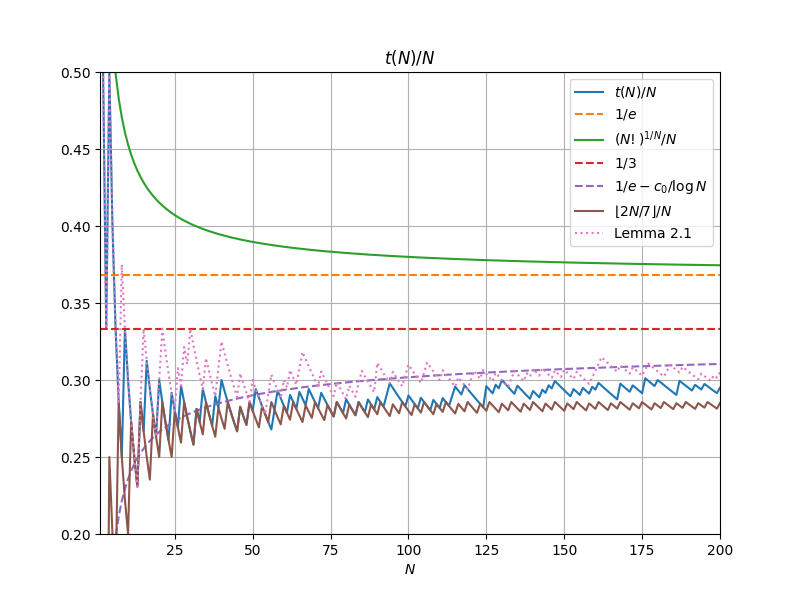
\includegraphics[width=0.8\textwidth]{newplot_200.png}
  \caption{The function $t(N)/N$ (blue) for $N \leq 200$, using the data from \href{https://oeis.org/A034258}{OEIS A034258}, as well as the trivial upper bound $(N!)^{1/N}/N$ (green), the improved upper bound from \Cref{upper-crit} (pink), which is asymptotic to \eqref{asym} (purple), and the function $\lfloor 2N/7 \rfloor/N$ (brown), which we show to be a lower bound for $N \neq 56$.  \Cref{main} implies that $t(N)/N$ is asymptotic to \eqref{asym} (purple), which in turn converges to $1/e$ (orange).  The threshold $1/3$ (red) is permanently crossed at $N=43632$. 
  }\label{fig1}
  \end{figure}
  
  \begin{figure}
    \centering
    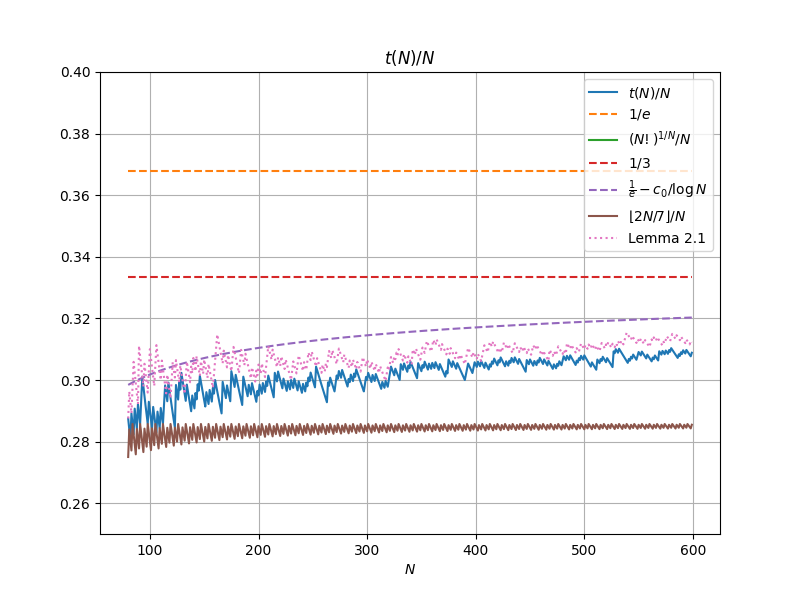
\includegraphics[width=0.8\textwidth]{newplot_600_all.png}
    \caption{A continuation of \Cref{fig1} to the region $80 \leq N \leq 599$. }\label{fig1-alt}
  \end{figure}
  
In this paper we answer all of these questions.

\begin{theorem}[Main theorem]\label{main} Let $N$ be a natural number.
\begin{itemize}
\item[(i)] If $N \neq 1,2,4$, then $t(N) \leq N/e$.
\item[(ii)]  If $N \neq 56$, then $t(N) \geq \lfloor 2N/7 \rfloor$.
\item[(iii)]  If $N \geq 43632$, then $t(N) \geq N/3$.  The threshold $43632$ is best possible.
\item[(iv)]  For large $N$, one has
  \begin{equation}\label{asym}
    \frac{t(N)}{N} = \frac{1}{e} - \frac{c_0}{\log N} + O\left( \frac{1}{\log^{1+c} N} \right)
  \end{equation}
for some constant $c>0$, where $c_0$ is the explicit constant
\begin{equation}\label{c0-def}
  \begin{split}
  c_0 &\coloneqq \frac{1}{e} \int_0^1 f_e(x)\ dx \\
  &= 0.30441901\dots
\end{split}
\end{equation}
and for any $\alpha>0$, $f_\alpha \colon (0,\infty) \to \R$ denotes the piecewise smooth function
\begin{equation}\label{falpha-def} 
  f_\alpha(x) \coloneqq \left\lfloor \frac{1}{x} \right\rfloor \log \frac{\lceil 1/\alpha x \rceil}{1/\alpha x}.
\end{equation}
In particular, \eqref{t1} and \eqref{Tbound} hold.  In fact the upper bound can be sharpened to
\begin{equation}\label{tna} 
  \frac{t(N)}{N} \leq \frac{1}{e} - \frac{c_0}{\log N} - \frac{c_1+o(1)}{\log^2 N} 
\end{equation}
for an explicit constant $c_1=0.75554808\dots$; see \Cref{upper-bound}.
\end{itemize}
\end{theorem}

For future reference, we observe the simple bounds
\begin{equation}\label{falpha-bound}
 \begin{split}
   0 \leq f_\alpha(x) &\leq \frac{1}{x} \log \frac{1/\alpha x+1}{1/\alpha x}\\
&= \frac{1}{x} \log\left( 1 + \alpha x \right) \\
&\leq \alpha
\end{split}
\end{equation}
for all $x>0$; in particular, $f_\alpha$ is a bounded function.  It however has an oscillating singularity at $x=0$; see \Cref{fig-mean}.

In \Cref{c0-app} we give some details on the numerical computation of the constant $c_0$.

\begin{remark}\label{old} In a previous version \cite{tao} of this manuscript, the weaker bounds
  $$ \frac{1}{e} - \frac{O(1)}{\log N} \leq \frac{t(N)}{N} \leq \frac{1}{e} - \frac{c_0+o(1)}{\log N}$$
were established, which were enough to recover \eqref{t1}, \eqref{Tbound}, and \Cref{main}(i). 
\end{remark}  

\begin{figure}
  \centering
  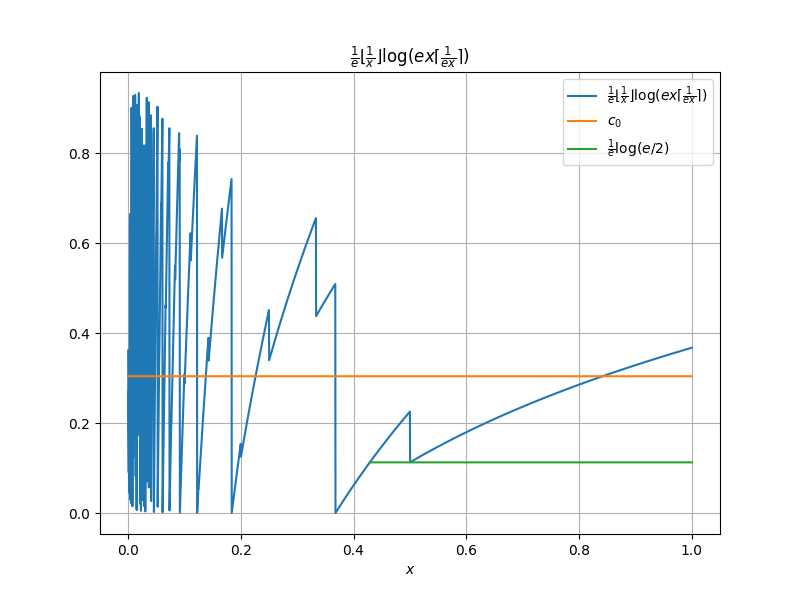
\includegraphics[width=0.8\textwidth]{integ.png}
  \caption{The piecewise continuous function $x\mapsto \frac{1}{e} f_e(x)$, together with its mean value $c_0 = 0.30441901\dots$ and the upper bound $\frac{\log(1+ex)}{ex}$.  The function exhibits an oscillatory singularity at $x=0$ similar to $\sin \frac{1}{x}$ (but it is always nonnegative and bounded). Informally, the function $f_e$ quantifies the difficulty that large primes in the factorization of $N!$ have in becoming slightly larger than $N/e$ after multiplying by a natural number.}\label{fig-mean}
\end{figure}

As one might expect, the proof of \Cref{main} proceeds by a combination of both theoretical analysis and numerical calculations.  Our main tools to obtain upper and lower bounds on $t(N)$ can be summarized as follows:

\begin{itemize}
  \item In \Cref{greedy-sec}, we discuss \emph{greedy algorithms} to construct subfactorizations, that provide quickly computable, though suboptimal, lower bounds on $t(N)$ for small and medium values;
  \item In \Cref{linprog-sec}, we present a \emph{linear programming} (or \emph{integer programming}) method that provides quite accurate upper and lower bounds on $t(N)$ for small and medium values of $N$;
  \item In \Cref{accounting-sec}, we introduce an \emph{accounting equation} linking the ``$t$-excess'' of a subfactorization with its ``$p$-surpluses'' at various primes, which provides an reasonable upper bound on $t(N)$ for all $N$, and is discussed in more detail in \Cref{accounting-sec};
  \item In \Cref{rearrange-sec}, we extend the \emph{rearrangement approach} from \cite{guy-selfridge} to give a computer-assisted proof that \Cref{main}(iii) holds for sufficiently large $N$.
  \item In \Cref{approx-sec}, we give \emph{modified approximate factorization} strategy, which provides lower bounds on $t(N)$, that become asymptotically quite efficient.
\end{itemize}


The final approach is significantly more complicated than the other four, but gives the most efficient lower bounds in the asymptotic limit $N \to \infty$.  The key idea is to start with an approximate factorization
$$ N! \approx \left(\prod_{j \in I} j\right)^A$$
for some relatively small natural number $A$ (e.g., $A = \lfloor \log^2 N \rfloor$) and a suitable set $I$ of natural numbers greater than or equal to $t$; there is some freedom to select parameters here, and we will take $I$ to be the natural numbers in $(t, t(1+\sigma)]$ that are $3$-rough (coprime to $6$), where $t$ is the target lower bound for $t(N)$ we wish to establish, and $\sigma \coloneqq \frac{3N}{tA}$ is chosen to bring the number of terms in the approximate factorization close to $N$.  With this choice of $I$, this product contains approximately the right number of copies of $p$ for medium-sized primes $p$; but it has the ``wrong'' number of copies of large primes, and is also constructed to avoid the ``tiny'' primes $p=2,3$.  One then performs a number of alterations to this approximate factorization to correct for the ``surpluses'' or ``deficits'' at various primes $p>3$, using the supply of available tiny primes $p=2,3$ as a sort of ``liquidity pool'' to efficiently reallocate primes in the factorization.  A key point will be that the incommensurability of $\log 2$ and $\log 3$ (i.e., the irrationality of $\log 3/\log 2$) means that the $3$-smooth numbers (numbers of the form $2^n 3^m$) are asymptotically dense (in logarithmic scale), allowing for other factors to be exchanged for $3$-smooth factors with little loss\footnote{The weaker results alluded to in \Cref{old} only used the prime $2$ as a supply of ``liquidity'', and thus encountered inefficiencies due to the inability to ``make change'' when approximating another factor by a power of two.}.

\subsection{Author contributions and data}

This project was initially conceived as a single-author manuscript by Terence Tao, but since the release of the initial preprint \cite{tao}, grew to become a collaborative project organized via the Github repository \cite{github}, which also contains the supporting code and data for the project.  The contributions of the individual authors, according to the CRediT categories\footnote{\url{https://credit.niso.org/}}, are as follows:

\begin{itemize}
\item Boris Alexeev: ...
\item Evan Conway: ...
\item Andrew Sutherland: ...
\item Terence Tao: Conceptualization, Formal Analysis, Methodology, Project Administration, Visualization, Writing -- original draft, Writing -- review \& editing.
\item Markus Uhr: Initial conception and implementation of linear programming, numerical analysis.
\item Kevin Ventullo: Software
\end{itemize}

\subsection{Acknowledgments}

TT is supported by NSF grant DMS-2347850.  We thank Thomas Bloom for the web site \url{https://www.erdosproblems.com}, where the author learned of this problem, as well as Bryna Kra and Ivan Pan for  corrections.


\section{Notation and basic estimates}

We use the usual asymptotic notation $X = O(Y)$, $X \ll Y$, or $Y \gg X$ to denote an inequality of the form $|X| \leq CY$ for some absolute constant $C$.  We also write $X \asymp Y$ for $X \ll Y \ll X$. For effective estimates, we will use the more precise notation $O_{\leq}(Y)$ to denote any quantity whose magnitude is bounded by exactly at most $Y$. We also use $O_{\leq}(Y)^+$ to denote a quantity of size $O_{\leq}(Y)$ that is also non-negative, that is to say it lies in the interval $[0,Y]$.  We also use $o(X)$ to denote any quantity bounded in magnitude by $c(N) X$, for some $c(N)$ that goes to zero as $N \to \infty$.

If $S$ is a statement, we use $1_S$ to denote its indicator, thus $1_S=1$ when $S$ is true and $1_S=0$ when $S$ is false.  If $x$ is a real number, we use $\lfloor x \rfloor$ to denote the greatest integer less than or equal to $x$, and $\lceil x \rceil$ to be the least integer greater than or equal to $x$.

Throughout this paper, the symbol $p$ (or $p_0$, $p_1$, etc.) is always understood to be restricted to be prime.  
We use $(a,b)$ to denote the greatest common divisor of $a$ and $b$, $a|b$ to denote the assertion that $a$ divides $b$, and $\pi(x) = \sum_{p \leq x} 1$ to denote the usual prime counting function.

We use $\nu_p(a/b) = \nu_p(a)-\nu_p(b)$ to denote the $p$-adic valuation of a positive natural number $a/b$, that is to say the number of times $p$ divides the numerator $a$, minus the number of times $p$ divides the denominator $b$.  For instance, $\nu_2(32/27)=5$ and $\nu_3(32/27)=-3$. 
If one applies a logarithm to the fundamental theorem of arithmetic, one obtains the identity
\begin{equation}\label{ftoa}
  \sum_p \nu_p(r) \log p = \log r
\end{equation}
for any positive rational $r$.  

For a natural number $n$, we can write
\begin{equation}\label{nup-form} 
  \nu_p(n) = \sum_{j=1}^\infty 1_{p^j|n}.
\end{equation}
Upon taking partial sums, we recover Legendre's formula
\begin{equation}\label{legendre}
  \nu_p(N!) = \sum_{j=1}^\infty \left\lfloor \frac{N}{p^j} \right\rfloor = \frac{N - s_p(N)}{p-1}
\end{equation}
where $s_p(N)$ is the sum of the digits of $N$ in the base $p$ expansion.

Given a putative factorization $\tuple$ of $N!$,  
we refer to the quantity $\nu_p\left( \frac{N!}{\prod \tuple} \right)$ as the \emph{$p$-surplus} of $\tuple$ with respect to the target $N!$, and similarly refer to the negative $-\nu_p\left( \frac{N!}{\prod \tuple} \right) = \nu_p\left( \frac{\prod \tuple}{N!} \right)$ of this surplus as the \emph{$p$-deficit}, with the multiset being \emph{$p$-balanced} if the $p$-surplus (or $p$-deficit) is zero.  Thus, a factorization of $N!$ is achieved if and only if one is balanced at every prime $p$, whereas a subfactorization is achieved if one is either in balance or surplus at every prime $p$.

To bound the factorial, we have the explicit Stirling approximation \cite{robbins}
\begin{equation}\label{stirling}
\log N! = N \log N - N + \log \sqrt{2\pi N} + O_\leq^+\left(\frac{1}{12N}\right),
\end{equation}
valid for all natural numbers $N$. 

\subsection{Approximation by \texorpdfstring{$3$}{3}-smooth numbers} 

The primes $2,3$ will play a special role\footnote{One could also run analogous arguments with other sets of tiny primes; for instance, the initial version \cite{tao} of this paper only utilized the prime $2$ in this fashion.} in this paper and will be referred to as \emph{tiny primes}. 
Call a natural number \emph{$3$-smooth} if it is the product of tiny primes, i.e., it is of the form $2^n 3^m$ for some natural numbers $n,m$, and \emph{$3$-rough} if it is not divisible by any tiny prime, that is to say it is coprime to $6$.  Given a positive real number $x$, we use $\lceil x \rceil^{\langle 2,3 \rangle}$ to denote the smallest $3$-smooth number greater than or equal to $x$.  For instance, $\lceil 5 \rceil^{\langle 2,3 \rangle} = 6$ and $\lceil 10 \rceil^{\langle 2,3 \rangle} = 12$.  

It will be convenient to introduce a variant of this quantity that is close to a power\footnote{The significance of the base $12$ is that the $3$-smooth portion $2^{\nu_2(N!)} 3^{\nu_3(N!)}$ of $N!$, which serves as our ``liquidity pool'', is approximately $2^N 3^{N/2} = \sqrt{12}^{N}$; see \eqref{legendre} below.  This makes $\log \sqrt{12}$ a natural ``unit of currency'' in which to conduct various factor exchanges, with various integer linear combinations of $\log 2$ and $\log 3$ usable as ``small change'' to approximate quantities that are not integer multiples of $\log \sqrt{12} = \log 2 + \frac{1}{2} \log 3$.} of $12$.  If $1 \leq L \leq x$ is an additional real parameter, we define
\begin{equation}\label{fancy-kappa-def}
  \lceil x \rceil^{\langle 2,3\rangle}_L \coloneqq 12^a \lceil x/12^a \rceil^{\langle 2,3 \rangle}
\end{equation}
for any real $x \geq L \geq 1$, where $a \coloneqq \lfloor \frac{x/L}{\log 12} \rfloor$ is the largest integer such that $12^a \leq x/L$.  

For any $L \geq 1$, let $\kappa_L$ be the least quantity such that
\begin{equation}\label{kappa-def}  
  x \leq \lceil x \rceil^{\langle 2,3\rangle} \leq \exp(\kappa_L) x 
\end{equation}
holds for all $x \geq L$; see \Cref{fig:nextsmooth}.  In \Cref{power-sec} we establish the following facts:

\begin{figure}
  \centering
  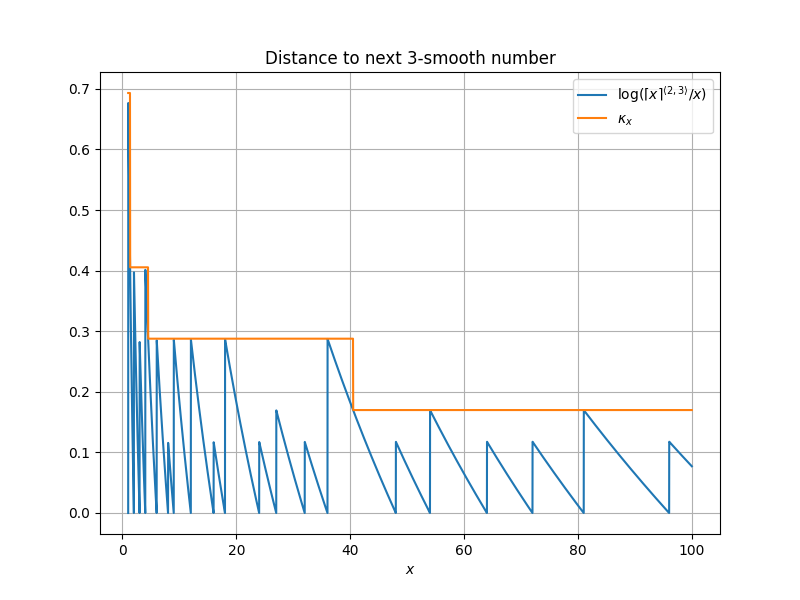
\includegraphics[width=0.8\textwidth]{next_smooth.png}
  \caption{The function $\log \frac{\lceil x \rceil^{\langle 2,3 \rangle}}{x}$, compared against $\kappa_x$. 
  }\label{fig:nextsmooth}
  \end{figure}


\begin{lemma}[Approximation by $3$-smooth numbers]\label{power-lemma}\ 
\begin{itemize}
\item[(i)]  We have $\kappa_{4.5} = \log\frac{4}{3} = 0.28768\dots$ and $\kappa_{40.5} = \log \frac{32}{27} = 0.16989\dots$.
\item[(ii)]  For large $L$, one has $\kappa_L \ll \log^{-c} L$ for some absolute constant $c>0$.
\item[(iii)]  If $1 \leq L \leq x$ are real numbers, then
\begin{equation}\label{mod-kappa}
  x \leq \lceil x \rceil^{\langle 2,3\rangle}_L \leq \exp(\kappa_L) x 
\end{equation}
and for any $0 \leq \gamma < 1$ we have
\begin{equation}\label{12-2}
\frac{\nu_2(\lceil x \rceil^{\langle 2,3\rangle}_L) - 2 \gamma \nu_3(\lceil x \rceil^{\langle 2,3\rangle}_L)}{1-\gamma} \leq \frac{\log x  + \kappa^{(2)}_{L,\gamma} }{\log \sqrt{12}} 
\end{equation}
and
\begin{equation}\label{12-3}
\frac{2\nu_3(\lceil x \rceil^{\langle 2,3\rangle}_L) - \gamma \nu_2(\lceil x \rceil^{\langle 2,3\rangle}_L)}{1-\gamma} \leq \frac{\log x + \kappa^{(3)}_{L,\gamma} }{\log \sqrt{12}} 
\end{equation}
where
\begin{equation}\label{kappastar-2-def}
\kappa^{(2)}_{L,\gamma} \coloneqq \left(\frac{\log \sqrt{12}}{(1-\gamma)\log 2} - 1\right) \log(12L) + \frac{\kappa_L\log \sqrt{12}}{(1-\gamma) \log 2}
\end{equation}
\begin{equation}\label{kappastar-3-def}
  \kappa^{(3)}_{L,\gamma} \coloneqq \left(\frac{\log \sqrt{12}}{(1-\gamma)\log \sqrt{3}} - 1\right) \log(12L) + \frac{\kappa_L\log \sqrt{12}}{(1-\gamma)\log \sqrt{3}}.
\end{equation}
\end{itemize}
\end{lemma}

We remark that when $x$ is a power of $12$, the left-hand sides of \eqref{12-2}, \eqref{12-3} are both equal to $\frac{\log x}{\log \sqrt{12}}$; thus the estimates \eqref{12-2}, \eqref{12-3} are quite efficient asymptotically.

\subsection{Sums over primes}

We recall the effective prime number theorem from \cite[Corollary 5.2]{dusart}, which asserts that
\begin{equation}\label{pi-lower}
  \pi(x) \geq \frac{x}{\log x} + \frac{x}{\log^2 x}
\end{equation}
for $x \geq 599$ and
\begin{equation}\label{pi-upper}
  \pi(x) \leq \frac{x}{\log x} + \frac{1.2762 x}{\log^2 x}
\end{equation}
for $x >1$.  

We will also need to control sums of somewhat oscillatory functions over primes, for which the bounds in \eqref{pi-lower}, \eqref{pi-upper} are of insufficient strength. Let $y<x$ be real numbers. Given a function $b \colon (y,x] \to \R$, its \emph{total variation}
$\|b\|_{\mathrm{TV}(y,x]}$ is defined as the supremum of the quantities $\sum_{j=0}^{J-1} |b(x_{j+1})-b(x_j)|$ for $y < x_0 \leq \dots \leq x_J \leq x$, and the \emph{augmented total variation} $\|b\|_{\mathrm{TV}^*(y,x]}$ is defined as
$$
\|b\|_{\mathrm{TV}^*(y,x]}
\coloneqq |b(y^+)| + |b(x)| + \|b\|_{\mathrm{TV}(y,x]},$$
$b(y^+) \coloneqq \lim_{t \to y^+} b(t)$ denotes the right limit of $b$ at $y$ (which exists if $b$ is of finite total variation).  Equivalently, $\|b\|_{\mathrm{TV}^*(y,x]}$ is the total variation of $b$ if extended by zero outside of $(y,x]$. The indicator function $1_{(y,x]}$ clearly has an augmented total variation of $2$.

We will use this augmented total variation to control sums over primes.  More precisely, in \Cref{primes-sec} we will show

\begin{lemma}[Effective bounds for oscillatory sums over primes]\label{osc-lemma}  Let $1423 \leq y \leq x$, and let $b: (y,x] \to \R$ be of bounded total variation.  Then we have the bound
\begin{equation}\label{bv-exact}
    \sum_{y < p \leq x} b(p) \log p = \int_y^x \left(1-\frac{2}{\sqrt{t}}\right) b(t)\ dt + O_{\leq}(\|b\|_{\mathrm{TV}^*(y,x]} E(x))
\end{equation}
where the error function $E(x)$ is defined as
\begin{equation}\label{tilde-e}
  E(x) \coloneqq 0.95 \sqrt{x} + 3.83 \times 10^{-9} x.
\end{equation}
In particular one has
\begin{equation}\label{pix}
  \pi(x) - \pi(y) = \int_y^x \left(1-\frac{2}{\sqrt{t}}\right)\frac{dt}{\log t} + O_\leq\left(2 \frac{E(x)}{\log y}\right);
\end{equation}
estimating
$$ 1-\frac{2}{\sqrt{y}} \leq 1-\frac{2}{\sqrt{t}} \leq 1$$
and using the convexity of $t \mapsto \frac{1}{\log t}$, we obtain the upper bound
\begin{equation}\label{pixy-upper}
 \pi(x) - \pi(y) \leq \frac{x-y}{2\log y} + \frac{x-y}{2\log x} + 2 \frac{E(x)}{\log y}
\end{equation}
and the lower bound
\begin{equation}\label{pixy-lower}
  \pi(x) - \pi(y) \geq \left(1-\frac{2}{\sqrt{y}}\right) \frac{x-y}{\log \frac{x+y}{2}} - 2 \frac{E(x)}{\log y}.
\end{equation}
For non-negative $b$ and the trivial inequalities
$$ \frac{b(p) \log p}{\log x}  \leq b(p) \leq \frac{b(p) \log p}{\log y} $$
we similarly obtain the upper bound
\begin{equation}\label{bv-upper}
   \sum_{y < p \leq x} b(p) \leq \frac{1}{\log y} \int_y^x b(t)\ dt + \|b\|_{\mathrm{TV}^*(y,x]} \frac{E(x)}{\log y}
\end{equation}
and the lower bound
\begin{equation}\label{bv-lower}
  \sum_{y < p \leq x} b(p) \leq \frac{1-\frac{2}{\sqrt{y}}}{\log x} \int_y^x b(t)\ dt - \|b\|_{\mathrm{TV}^*(y,x]} \frac{E(x)}{\log x}.
\end{equation}
One can also replace all occurrences of $E(x)$ here by the classical error term $O(x \exp(-c \sqrt{\log x}))$ for some absolute constant $c>0$ (in which case the $\frac{2}{\sqrt{t}}$ type terms can be absorbed into the error term).
\end{lemma}

We remark that the accuracy in \eqref{bv-exact}, \eqref{pix} in particular is on par with what would be provided by the Riemann hypothesis, as long as $x$ is not too large (e.g., $x \leq 10^{18}$).  The other estimates in this lemma are not quite as precise, but still adequate for our applications.  The error term $E(x)$ can be improved somewhat for large $x$ (see \eqref{etil-def}), but this simplified version will suffice for our analysis (in particular, the contribution of the second term in \eqref{tilde-e} will be negligible for our applications).  We make the easy remark that $E(x)$ is non-decreasing in $x$, while $E(x)/x$ is non-increasing.

\section{Greedy algorithms}\label{greedy-sec}

The following simple greedy algorithm gives reasonably good performance to obtain large $t$-admissible subfactorizations $\tuple$ of $N!$ for a given choice of $t$ and $N$:

\begin{enumerate}
\item[(0)] Initialize $\tuple$ to be the empty multiset. 
\item[(1)] If $\tuple$ is not a factorization, locate the largest prime $p$ which is currently in surplus: $\nu_p(N!/\prod \tuple) > 0$. 
\item[(2)] If $N! / \prod \tuple$ contains a multiple of $p$ that is greater than or equal to $t$, locate the smallest such multiple, add it to $\tuple$, and return to Step 1.  Otherwise, \texttt{HALT} the algorithm. 
\end{enumerate}

This procedure clearly halts in finite time to produce a $t$-admissible subfactorization of $N!$.  For instance, applying this procedure with $N=9$, $t=3$ produces the $3$-admissible subfactorization
$$ \{7 \times 1, 5 \times 1, 3 \times 1, 3 \times 1, 3 \times 1, 3 \times 1, 2 \times 2, 2 \times 2, 2 \times 2 \}$$
which recovers the bound $t(9) \geq 3$ from \Cref{nine} (though with a slightly different subfactorization, in which the $8$ is replaced by $4$).

This procedure is efficient for small $N$, for instance attaining the exact value of $t(N)$ for all $N \leq 79$, though it begins to degrade for larger $N$; see \Cref{fig-zoom}.  The performance is also respectable (though not optimal) for medium $N$; for instance, when $N=3 \times 10^5$ and $t=N/3$, it locates a $t$-admissible subfactorization of $N!$ of cardinality $N+372$, which is close to the linear programming limit of $N+455$ established in the next section.

{\bf discuss modifications to the algorithm to make it perform both faster and more accurately}

In order to get this algorithm to validate all $8 \times 10^4 \leq N \leq 10^{11}$ on commodity hardware in a reasonable amount of time, two major modifications were implemented. 

First, when trying to improve an inequality $t(N) \geq \lambda N$ for all $N$ in some range, one can avoid running the algorithm for every single $N$ in that range by instead proving a stronger inequality on a sparse subset. Namely, if one can show that $t(N_0) \geq (\lambda + \eps)N_0$, it follows that $t(N) \geq \lambda N$ for all $N \in \left[N_0, (1+\frac{\eps}{\lambda})N_0\right)$. If one can fix $\eps$, this reduces a brute force check of every value in a range of length $L$ to checking just $\log_{1+\frac{\eps}{\lambda}}(L)$ values. From the estimates in Section 1, one would expect to be able to take $\eps = \frac{1}{e}-\lambda$ asymptotically; in practice the algorithm uses slightly smaller values. 

The other major modification is related to Step (2) in the above algorithm, where one is searching for the least value of $c$ such that $cp\geq t$ and $c$ can be constructed from the remaining factors. In practice, the algorithm pre-computes and store information about all such candidates; absent any further heuristics, this amounts to storing information about all integers less than $N$, which becomes prohibitively expensive for large $N$. The key observation is that any such $c$ must satisfy a further arithmetic condition, namely that $\frac{cL(c)}{S(c)} < t$. By only storing information about $c$ which satisfy this condition, the memory footprint is reduced by several orders of magnitude.

By using the greedy method, \Cref{main}(ii) can be verified for $N \leq 3 \times 10^5$, and \Cref{main}(iii) can be verified for $8 \times 10^4 \leq N \leq 10^{11}$.    Thus, to resolve these claims, it remains to only establish \Cref{main}(iii) in the regime $43632 \leq N < 8 \times 10^4$ and $N > 10^{11}$, and also to show that this claim fails for $N=43631$.

{\bf would be nice to have some data to plot on the greedy algorithm performance for the range $10^4 \leq N \leq 10^{11}$}

\section{Linear programming}\label{linprog-sec}

A $t$-admissible subfactorization of $N!$ can also be viewed as a product
$$ \prod_{j \geq t} j^{m_j}$$
for some non-negative integers $m_j$ that obey the linear constraints
\begin{equation}\label{constraints}
  \sum_{j \geq t} m_j \nu_p(j) \leq \nu_p(N!)
\end{equation}
for all primes $p$.  Thus, we have an alternative description of $t(N)$:

\begin{proposition}  For any $N \geq 1$, $t(N)$ is the largest quantity $t$ for which there is a solution to the infinite integer program \eqref{constraints}, where $m_j$ are constrained to be non-negative integers with
$$ \sum_j m_j \leq N.$$
\end{proposition}

This proposition suggests the possibility of using linear programming (or integer programming) methods to provide upper and lower bounds on $t(N)$. An immediate issue for computational purposes is that this program involves an infinite number of variables $m_j$.  However, observe that any $j$ not dividing $N!$ cannot be used; and furthermore if $j$ contains a strictly smaller factor that is at least $t$, then it could be replaced by that factor while still generating a $t$-admissible subfactorization of $N$.  As a consequence of these two facts, $j$ can be restricted to a finite set $J_{t,N}$ of the numbers $t \leq j \leq \max(N,t^2)$ dividing $N!$ with no proper factors greater than or equal to $t$.  This makes the integer program finite (though somewhat large), and in particular computable for small $N$, such as $N \leq 10^4$.  By relaxing the integer program to a linear program, one can also obtain upper and lower bounds as follows:

\begin{itemize}
  \item If one uses linear programming to maximize the quantity $\sum_{j \in J_{t,N}} m_j$ for non-negative \emph{reals} $m_j$ subject to the constraints \eqref{conditions}, and $\sum_{j \in J_{t,N}} \lfloor m_j \rfloor \geq N$, then $\prod_{j \in J_{t,N}} j^{\lfloor m_j \rfloor}$ represents a $t$-admissible subfactorization of $N!$ that witnesses $t(N) \geq t$.
  \item If the dual linear program of finding non-negative reals $w_p$ for each prime $p \leq N$ that satisfy the dual constraints
  \begin{equation}\label{pj}
    \sum_p w_p \nu_p(j) \geq 1
   \end{equation}
   for all $j \in J_{t,N}$ as well as
   \begin{equation}\label{hyp}
    \sum_p w_p \nu_p(N!) < N,
    \end{equation}
    then by multiplying \eqref{constraints} by $w_p$ and summing over $p \leq N$, we see that these constraints force $\sum_{j \in J_{t,N}} m_j < N$, and hence $t(N) < t$.
\end{itemize}

By the duality of linear programming, these upper bounds and lower bounds would match if the constraint $\sum_{j \in J_{t,N}} \lfloor m_j \rfloor \leq N$ in the lower bound were replaced with the linear constraint $\sum_{j \in J_{t,N}} m_j \leq N$.

In practice, the linear programming method is extremely accurate in upper and lower bounding $t(N)$; for instance, they give the exact value of $t(N)$ for all $N \leq 600$, with the sole exception of $N=155$, where the linear programming bounds instead give $45 \leq t(155) \leq 46$.  In this case, the (slower) integer programming method can be deployed to verify that $t(155)=45$.


However, the large size of $J_{t,N}$ renders a direct application of the linear programming approach computationally expensive once $N$ exceeds $10^3$ or so.  For the purpose of establishing lower bounds, one can of course reduce this set arbitrarily; we have found a good choice to be the integers between $t$ and $N$.  For the dual problem, we are also able to make such a reduction, under the additional hypotheses that the weights $w_p$ are non-decreasing:
  
\begin{lemma}[Linear programming bound]\label{lp-upper}  Let $N$ be an natural number and $1 \leq t \leq N/2$.  Suppose for each prime $p \leq N$, one has a non-negative real number $w_p$ which is weakly non-decreasing in $p$ (thus $w_p \leq w_{p'}$ when $p \leq p'$), and such that \eqref{pj} holds
  for all $t \leq j \leq N$, and such that \eqref{hyp} also holds.
\end{lemma}
  
\begin{proof}
By the previous remarks, it will suffice to show that the bound \eqref{pj} in fact holds for all $j \geq t$, not just for $t \leq j \leq N$.  Indeed, if this were not the case, consider the first $j \geq t$ where \eqref{pj} fails.  Take a prime $p$ dividing $j$ and replace it by a prime in the interval $[p/2,p)$ which exists by Bertrand's postulate (or remove $p$ entirely, if $p=2$); this creates a new $j'$ in $[j/2,j)$ which is still at least $t$.  By the weakly decreasing hypothesis on $w_p$, we have
  $$ \sum_p w_p \nu_p(j) \geq \sum_p w_p \nu_p(j')$$
  and hence by the minimality of $j$ we have
  $$ \sum_p w_p \nu_p(j) > 1, $$
  a contradiction.
\end{proof}
  
We have found empirically that using linear programming to maximize the left-hand side of \eqref{hyp} subject to \eqref{pj} for $t \leq j \leq N$ tends to generate weights $w_p$ that are in fact weakly decreasing, so that a rigorous upper bound $t(N) < t$ can be established by this method without needing to expand the linear program to all $j \in J_{t,N}$.  With this technique, the linear programming method can now be run to cover all $N \leq 10^4$ with the exception of $N=155,765,1528,1618,1619,2574,2935,3265,5122,5680,9633$, but in these cases $t(N)$ can be computed exactly by integer programming; see \cite{github} and \Cref{fig-long}.

One can also use this method to accurately bound subfactorizations of $N!$ for larger $N$, although the runtime becomes slow.  For instance, with $N = 3 \times 10^5$ and $t = N/3 = 10^5$, \Cref{lp-upper} can be used to show that any $t$-admissible factorization has cardinality at most $N+455$, while the lower bound linear program produces a $t$-admissible factorization of exactly this cardinality.  This demonstrates \Cref{main}(ii), (iii) for this value of $N$.  The linear programming method can also establish \Cref{main}(iii) in the range $43632 \leq N \leq 8 \times 10^4$, but show that this conjecture fails for $N = 43631$; it also holds for $N=41006$, but fails for all smaller $N$ except for $N=1,2,3,4,5,6,9$.  When combined with the greedy algorithm computations, this resolves \Cref{main}(ii), (iii) except in the asymptotic range $N > 10^{11}$, where it suffices to establish the lower bound $t(N) \geq N/3$.

{\bf more discussion here}


\begin{figure}
  \centering
  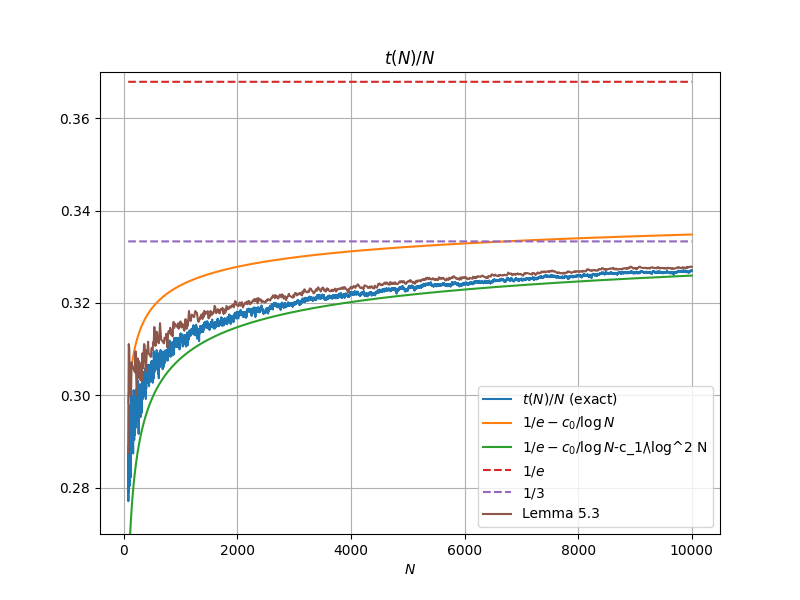
\includegraphics[width=0.5\textwidth]{longplot.png}
  \caption{$t(N)/N$ for $80 \leq N \leq 10^4$, obtained via linear programming in most cases (and integer programming in some exceptional cases).  The upper bound from \Cref{upper-crit} is surprisingly sharp, as is the refined asymptotic $1/e - c_0/\log N - c_1/\log^2 N$, though the cruder asymptotics $1/e$ or $1/e - c_0/\log N$ are significantly poorer approximations.}
  \label{fig-long}
  \end{figure}

  \begin{figure}
    \centering
    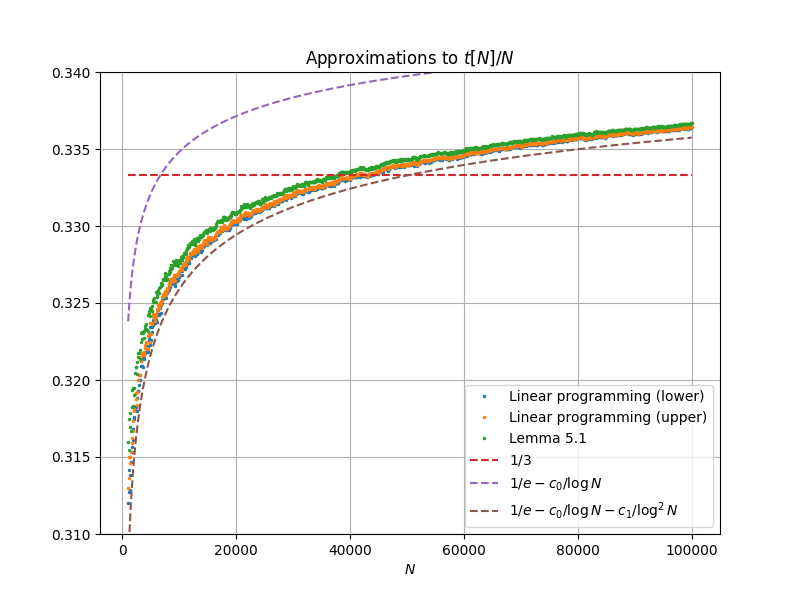
\includegraphics[width=0.5\textwidth]{longerplot.png}
    \caption{Upper and lower bounds $t(N)/N$ obtained by linear programming for some randomly sampled $10^3 \leq N \leq 10^5$. The refined asymptotic $1/e - c_0/\log N - c_1/\log^2 N$ is now a slight underestimate, hinting at further terms in the asymptotic expansion.}
    \label{fig-longer}
    \end{figure}

    
    \begin{table}[ht]
      \centering
      \begin{tabular}{|c|c|c|c|c|}
      \hline
      $N$ & $t(N)_-$ & $t(N)_+$ & \Cref{upper-crit} & $\frac{N}{e}-\frac{c_0 N}{\log N} - \frac{c_1 N}{\log^2 N}$  \\
      \hline
$1 \times 10^5$ & $\num{33642}$ & $t(N)_- + 4$ & $t(N)_- + 26$ & $t(N)_- - \num{69}$ \\
$2 \times 10^5$ & $\num{67703}$ & $t(N)_- + 1$ & $t(N)_- + 36$ & $t(N)_- - \num{130}$ \\
$3 \times 10^5$ & $\num{101903}$ & $t(N)_- + 3$ & $t(N)_- + 42$ & $t(N)_- - \num{206}$ \\
$4 \times 10^5$ & $\num{136143}$ & $t(N)_- + 6$ & $t(N)_- + 43$ & $t(N)_- - \num{248}$ \\
$5 \times 10^5$ & $\num{170456}$ & $t(N)_- + 3$ & $t(N)_- + 46$ & $t(N)_- - \num{310}$ \\
$6 \times 10^5$ & $\num{204811}$ & $t(N)_- + 4$ & $t(N)_- + 47$ & $t(N)_- - \num{373}$ \\
$7 \times 10^5$ & $\num{239187}$ & $t(N)_- + 9$ & $t(N)_- + 54$ & $t(N)_- - \num{425}$ \\
$8 \times 10^5$ & $\num{273604}$ & $t(N)_- + 6$ & $t(N)_- + 64$ & $t(N)_- - \num{490}$ \\
$9 \times 10^5$ & $\num{308029}$ & $t(N)_- + 13$ & $t(N)_- + 70$ & $t(N)_- - \num{539}$ \\
\hline
$1 \times 10^6$ & $\num{342505}$ & $t(N)_- + 3$ & $t(N)_- + 62$ & $t(N)_- - \num{619}$ \\
$2 \times 10^6$ & $\num{687796}$ & $t(N)_- + 4$ & $t(N)_- + 87$ & $t(N)_- - \num{1180}$ \\
$3 \times 10^6$ & $\num{1033949}$ & $t(N)_- + 11$ & $t(N)_- + 107$ & $t(N)_- - \num{1736}$ \\
$4 \times 10^6$ & $\num{1380625}$ & $t(N)_- + 12$ & $t(N)_- + 122$ & $t(N)_- - \num{2286}$ \\
$5 \times 10^6$ & $\num{1727605}$ & $t(N)_- + 4$ & $t(N)_- + 126$ & $t(N)_- - \num{2763}$ \\
$6 \times 10^6$ & $\num{2074962}$ & $t(N)_- + 21$ & $t(N)_- + 152$ & $t(N)_- - \num{3326}$ \\
$7 \times 10^6$ & $\num{2422486}$ & $t(N)_- + 22$ & $t(N)_- + 165$ & $t(N)_- - \num{3819}$ \\
$8 \times 10^6$ & $\num{2770212}$ & $t(N)_- + 29$ & $t(N)_- + 177$ & $t(N)_- - \num{4316}$ \\
$9 \times 10^6$ & $\num{3118129}$ & $t(N)_- + 24$ & $t(N)_- + 173$ & $t(N)_- - \num{4834}$ \\
\hline
$1 \times 10^7$ & $\num{3466235}$ & $t(N)_- + 12$ & $t(N)_- + 179$ & $t(N)_- - \num{5392}$ \\
$2 \times 10^7$ & $\num{6952243}$ & $t(N)_- + 18$ & $t(N)_- + 234$ & $t(N)_- - \num{10284}$ \\
$3 \times 10^7$ & $\num{10444441}$ & $t(N)_- + 13$ & $t(N)_- + 253$ & $t(N)_- - \num{14975}$ \\
$4 \times 10^7$ & $\num{13940484}$ & $t(N)_- + 64$ & $t(N)_- + 354$ & $t(N)_- - \num{19582}$ \\
$5 \times 10^7$ & $\num{17439282}$ & $t(N)_- + 33$ & $t(N)_- + 356$ & $t(N)_- - \num{24124}$ \\
$6 \times 10^7$ & $\num{20940210}$ & $t(N)_- + 23$ & $t(N)_- + 381$ & $t(N)_- - \num{28610}$ \\
$7 \times 10^7$ & $\num{24442818}$ & $t(N)_- + 37$ & $t(N)_- + 415$ & $t(N)_- - \num{32996}$ \\
$8 \times 10^7$ & $\num{27946958}$ & $t(N)_- + 43$ & $t(N)_- + 445$ & $t(N)_- - \num{37417}$ \\
$9 \times 10^7$ & $\num{31452431}$ & $t(N)_- + 23$ & $t(N)_- + 428$ & $t(N)_- - \num{41882}$ \\
\hline
$1 \times 10^8$ & $\num{34958725}$ & $t(N)_- + 48$ & $t(N)_- + 482$ & $t(N)_- - \num{46039}$ \\
$2 \times 10^8$ & $\num{70064782}$ & $t(N)_- + 45$ & $t(N)_- + 644$ & $t(N)_- - \num{87837}$ \\
$3 \times 10^8$ & $\num{105218403}$ & $t(N)_- + 41$ & $t(N)_- + 752$ & $t(N)_- - \num{128227}$ \\
$4 \times 10^8$ & $\num{140401212}$ & $t(N)_- + 80$ & $t(N)_- + 887$ & $t(N)_- - \num{167495}$ \\
$5 \times 10^8$ & $\num{175605266}$ & $t(N)_- + 98$ & $t(N)_- + 972$ & $t(N)_- - \num{206175}$ \\
$6 \times 10^8$ & $\num{210825848}$ & $t(N)_- + 68$ & $t(N)_- + 1058$ & $t(N)_- - \num{244391}$ \\
$7 \times 10^8$ & $\num{246059851}$ & $t(N)_- + 89$ & $t(N)_- + 1147$ & $t(N)_- - \num{282167}$ \\
      \hline
\end{tabular}
\caption{For sample values of $N \in [10^5, 7 \times 10^8]$, the (remarkably precise) lower and upper bounds $t(N)_- \leq t(N) \leq t(N)_+$ obtained by linear programming, the (slightly weaker) upper bound on $t(N)$ from \Cref{upper-crit}, and the conjectural approximation $\frac{N}{e} - \frac{c_0 N}{\log N} - \frac{c_1N}{\log^2 N}$ (rounded to the nearest integer).}\label{long-table}
\end{table}

      
      
\section{Some upper bounds}

It is easy to check using \eqref{ftoa} that the weights $w_p \coloneqq \frac{\log p}{\log t}$ will obey the requirements \eqref{pj}, \eqref{hyp} as long as $0 > \log N! - N \log t$.  This recovers the trivial upper bound \eqref{trivial}.  By adjusting these weights at large primes, one can improve this bound as follows:

\begin{lemma}[Upper bound criterion]\label{upper-crit}  Suppose that $1 \leq t \leq N$ are such that
  \begin{equation}\label{contra}
     \sum_{\frac{t}{\lfloor\sqrt{t}\rfloor} < p \leq N} f_{N/t}(p/N) > \log N! - N \log t,
  \end{equation}
  where $f_{N/t}$ was defined in \eqref{falpha-def}.
  Then $t(N) < t$.
  \end{lemma}

\begin{proof} We introduce the weights
  $$ 
w_p \coloneqq  \begin{cases} 
  \frac{\log p}{\log t} & p  \leq \frac{t}{\lfloor \sqrt{t} \rfloor} \\
  \frac{\log p}{\log t} - \frac{\log \frac{\lceil t/p \rceil}{t/p}}{\log t} = 1 - \frac{\log \lceil t/p \rceil}{\log t} & p  > \frac{t}{\lfloor \sqrt{t} \rfloor}.
\end{cases}
$$
Clearly the $w_p$ are non-negative.  It will suffice to verify the conditions \eqref{pj}, \eqref{hyp}.  If $j \in J_{t,N}$ contains no prime factor $p > \frac{t}{\lfloor \sqrt{t} \rfloor}$, then from \eqref{ftoa} we have
$$ \sum_p w_p \nu_p(j) = \frac{\sum_p \nu_p(j) \log p}{\log t} = \frac{\log j}{\log t} \geq 1.$$
If $j \in J_{t,N}$ is of the form $j = mp_1$ where $p_1 > \frac{t}{\lfloor \sqrt{t} \rfloor}$ and $m$ contains no prime factor exceeding $\frac{t}{\lfloor \sqrt{t} \rfloor}$, then $m \geq \lceil t/p_1 \rceil$, and we have
\begin{align*}
\sum_p w_p \nu_p(j) &= \frac{\sum_p \nu_p(j) \log p}{\log t}
- \frac{\log \frac{\lceil t/p_1 \rceil}{t/p_1}}{\log t}\\
&= \frac{\log(mp_1)}{\log t} -  \frac{\log \frac{m}{t/p_1}}{\log t} \\
&= 1.
\end{align*}
Finally, if $j \in J_{t,N}$ is divisible by two primes $p_1, p_2 > {t}{\lfloor \sqrt{t} \rfloor}$ (possibly equal), then
\begin{align*}
  \sum_p w_p \nu_p(j) &\geq
  1 - \frac{\log \lceil t/p_1 \rceil}{\log t} + 1 - \frac{\log \lceil t/p_1 \rceil}{\log t} \\
  &\geq
  1 - \frac{\log \sqrt{t}}{\log t} + 1 - \frac{\log \sqrt{t}}{\log t} \\
  &= 1.
\end{align*}
Thus we have verified \eqref{pj} for all $j \in J_{t,N}$.  Finally, from \eqref{ftoa}, \eqref{legendre}, \eqref{contra} we have
\begin{align*}
  \sum_p w_p \nu_p(N!) &= \frac{\sum_p \nu_p(N!) \log p}{\log t} - \sum_{p > \frac{t}{\lfloor \sqrt{t} \rfloor}} \frac{\nu_p(N!) \log \frac{\lceil t/p \rceil}{t/p}}{\log t} \\
  &\geq \frac{\log N!}{\log t} -  \frac{\sum_{p > \frac{t}{\lfloor \sqrt{t} \rfloor}} \lfloor \frac{N}{p} \rfloor \log \frac{\lceil t/p \rceil}{t/p}}{\log t}\\
  &= \frac{\log N!}{\log t} - \frac{\sum_{p > \frac{t}{\lfloor \sqrt{t} \rfloor}} f_{N/t}(p/N)}{\log t} \\
  &< N,
\end{align*}
giving \eqref{hyp}.  The claim follows.
\end{proof}


In practice, \Cref{upper-crit} gives quite good upper bounds on $N$, especially when $N$ is large, although for medium $N$ the linear programming method is superior: see \Cref{fig1}, \Cref{fig1-alt}, \Cref{fig-zoom}.
    
\begin{figure}
  \centering
  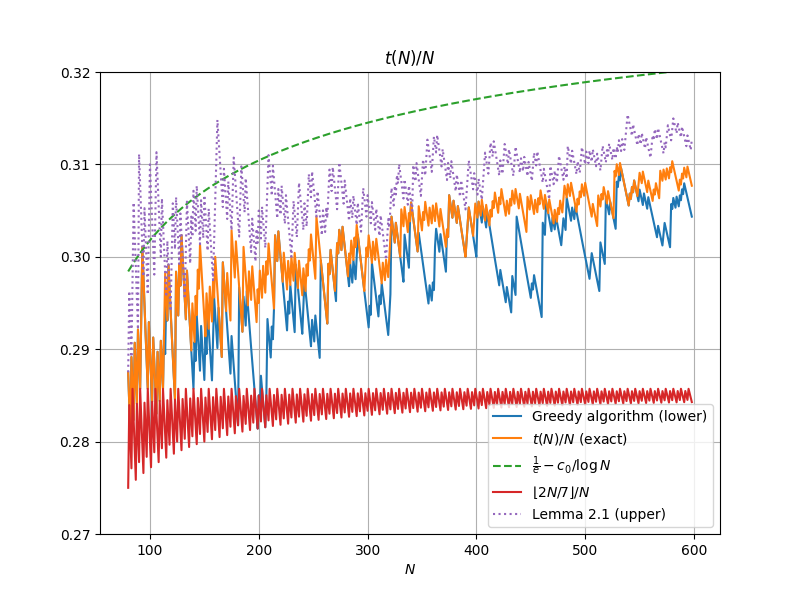
\includegraphics[width=0.8\textwidth]{newplot_600.png}
  \caption{An enlarged version of \Cref{fig1-alt}, displaying the lower bound from the greedy algorithm and the upper bound from \Cref{upper-crit}.  The linear programming upper and lower bounds are exact in this region, except for $N=155$ in which the upper bound is off by one.}\label{fig-zoom}
\end{figure}


\begin{figure}
  \centering
  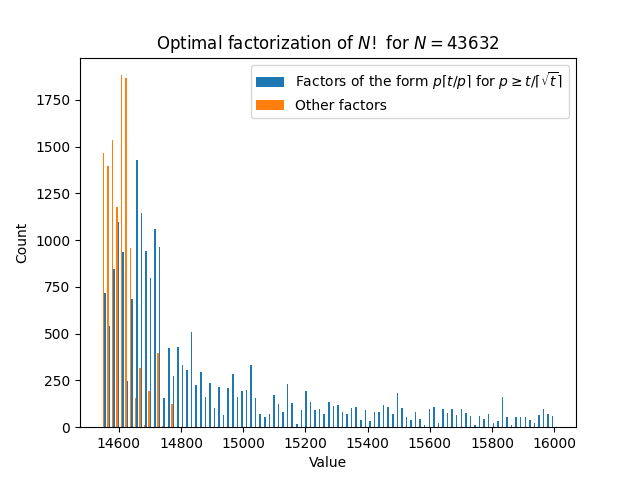
\includegraphics[width=0.8\textwidth]{factors.png}
  \caption{A histogram of an optimal factorization of $N!$ for $N=43632$, demonstrating that $t(N) = \lceil N/3\rceil = 14545$.  Of the $N$ factors, most ($\num{32147}$) of them are of the form $p \lceil t/p \rceil$ for $p > \frac{t}{\lfloor \sqrt{t} \rfloor}$, thus directly contributing to the left-hand side of \Cref{upper-crit}.  (The factors arising from very large primes are lie to the right of the displayed graph, as a long tail of the histogram.)  The remaining $\num{11485}$ factors stay close to $t(N)$, with the largest being $14941$.
  }\label{fig-factor}
  \end{figure}
  

We can now prove the upper bound portion of \Cref{main}(iv):

  \begin{proposition}\label{upper-bound}  For large $N$, one has
    $$ \frac{t(N)}{N} \leq \frac{1}{e} - \frac{c_0}{\log N} - \frac{c_1 + o(1)}{\log^2 N}$$
    where
    \begin{align}
      c'_1 &\coloneqq \frac{1}{e} \int_0^1 f_e(x) \log \frac{1}{x}\ dx = 0.3702015\dots \label{c1p-def}\\
      c''_1 &\coloneqq \sum_{k=1}^\infty \frac{1}{k}  \log\left( \frac{e}{k} \left\lceil \frac{k}{e} \right\rceil \right) \approx 1.6796\label{c1pp-def}\\
      c_1 &\coloneqq c'_1 + c_0 c''_1 - ec_0^2/2 \approx 0.75554808.\label{c1-def}
    \end{align}
  \end{proposition}

We discuss the numerical evaluation of these constants in \Cref{c0-app}.

  Numerically, this bound is a reasonably good approximation for medium-sized $N$, see \Cref{fig-long}, \Cref{fig-longer}, although it may be possible to improve the approximation further with additional terms.  Based on these numerics it seems natural to conjecture that one in fact has
  $$\frac{t(N)}{N} = \frac{1}{e} - \frac{c_0}{\log N} - \frac{c_1 + o(1)}{\log^2 N}$$
as $N \to \infty$.
    
    \begin{proof}  We apply \Cref{upper-crit} with
      $$ t \coloneqq \frac{1}{e} - \frac{c_0}{\log N} - \frac{c_1-\eps}{\log^2 N}$$
    for a given small constant $\eps>0$.  From Taylor expansion of the logarithm and the Stirling approximation \eqref{stirling} one sees that
    $$ \log N! - N \log t = ec_0 \frac{N}{\log N} + (ec_1 - \frac{1}{2} e^2 c_0^2 - e\eps+o(1)) \frac{N}{\log^2 N}$$
    so it will suffice to establish the lower bound
    \begin{equation}\label{targ-sum}
      \sum_{\frac{t}{\lfloor\sqrt{t}\rfloor} < p \leq N} f_{N/t}(p/N) \geq ec_0 \frac{N}{\log N} + (ec_1 - \frac{1}{2} e^2 c_0^2 - e \eps + o(1)) \frac{N}{\log^2 N}
    \end{equation}
    for $N$ sufficiently large depending on $\eps$.

    For $N$ large enough, we have $\frac{t}{\lfloor\sqrt{t}\rfloor} \leq \frac{N}{\log^3 N}$.
    On the interval $[1/\log^3 N,1]$, the piecewise smooth function $f_{N/t}$ is bounded by $O(1)$ thanks to \eqref{falpha-bound}, and has an (augmented) total variation of $O(\log^3 N)$; the same is then true for the rescaled function $x \mapsto f_{N/t}(x/N)$ on $[N/\log^3 N,1]$.   This implies that $x \mapsto \frac{1}{\log x} f_{N/t}(x/N)$ has an (augmented) total variation of $O(\log^2 N)$.
   By \Cref{osc-lemma} (with classical error term), we conclude that the left-hand side of \eqref{targ-sum} is at least
    $$ \int_{N/\log^3 N}^N f_{N/t}(x/N) \frac{dx}{\log x} + O\left( N \exp(-c\sqrt{\log N}) \right)$$
    for some $c>0$.  Performing a change of variable, we reduce to showing that
    $$  \int_{1/\log^3 N}^1 f_{N/t}(x) \frac{\log N}{\log(Nx)}\ dx 
    \geq  ec_0 + \frac{ec_1 - \frac{1}{2} e^2 c_0^2 - e \eps + o(1)}{\log N}.$$
    By Taylor expansion, we have
    $$ \frac{\log N}{\log(Nx)} = 1 + \frac{\log \frac{1}{x}}{\log N}  + o\left(\frac{1}{\log N}\right)$$
    and from dominated convergence we have
  $$
  \int_{1/\log^3 N}^1 f_{N/t}(x) \log \frac{1}{x}\ dx = ec'_1 + o(1)$$
and hence by definition of $c_1$, we reduce to showing that
$$  \int_{1/\log^3 N}^1 f_{N/t}(x)\ dx 
\geq  ec_0 + \frac{ec_0 c''_1 - e^2 c_0^2 - e\eps + o(1)}{\log N}.$$
By performing a rescaling by $N/et = 1 + \frac{ec_0+o(1)}{\log N}$, the left-hand side may be written as
$$ \left(1 - \frac{ec_0+o(1)}{\log N}\right) \int_{N/et\log^3 N}^{N/et}
\left\lfloor \frac{N/et}{x} \right\rfloor \log\left(ex \left\lceil \frac{1}{ex} \right\rceil \right) $$
so it will suffice to show that
$$
\int_{N/et\log^3 N}^{N/et}
\left\lfloor \frac{N/et}{x} \right\rfloor \log\left(ex \left\lceil \frac{1}{ex} \right\rceil \right)\ dx \geq ec_0 + \frac{ec_0 c''_1 - e\eps + o(1)}{\log N}.$$
From \eqref{c0-def}, \eqref{falpha-bound} we have
$$ \int_{1/\log^2 N}^1 \left\lfloor \frac{1}{x} \right\rfloor \log\left(ex \left\lceil \frac{1}{ex} \right\rceil \right) = ec_0 - \frac{o(1)}{\log N}$$
it suffices to show that
$$
\int_{1/log^2 N}^{N/et}
\left(\left\lfloor \frac{N/et}{x} \right\rfloor - \left\lfloor \frac{1}{x} \right\rfloor\right) \log\left(ex \left\lceil \frac{1}{ex} \right\rceil \right)\ dx \geq \frac{ec_0 c'' - e\eps + o(1)}{\log N}.$$
Let $K$ be sufficiently large depending on $\eps$, then for $N$ sufficiently large depending on $K$ we can lower bound the left-hand side by
$$ \sum_{k=1}^K \int_{1/k}^{N/etk} \log\left(ex \left\lceil \frac{1}{ex} \right\rceil \right)\ dx;$$
since $\frac{N}{etk} = \frac{1}{k} + \frac{ec_0}{k \log N}$, we can lower bound this (using the irrationality of $e$) by
$$ \frac{ec_0+o(1)}{\log N} \sum_{k=1}^K \frac{1}{k} \log\left(\frac{e}{k} \left\lceil \frac{k}{e} \right\rceil\right)$$
for sufficiently large $N$.  Since the sum here can be made arbitrarily close to $c''_0$ by increasing $K$, we obtain the claim.
\end{proof}
    
We can now establish \Cref{main}(i): 

\begin{proposition}\label{tne} One has $t(N)/N < 1/e$ for $N \neq 1,2,4$.
\end{proposition}

\begin{proof}  From existing data on $t(N)$ (or the linear programming method) one can verify this claim for $N < 80$ (see \Cref{fig1}), so we assume that $N\geq 80$.
  
Applying \Cref{upper-crit} and \eqref{stirling}, it suffices to show that
\begin{equation}\label{base-test-ineq}
   \sum_{p \geq \frac{N/e}{\lfloor\sqrt{N/e}\rfloor}} f_{e}(p/N) > \frac{1}{2} \log(2\pi N) + \frac{1}{12N}.
\end{equation}
This may be easily verified numerically in the range $80 \leq N \leq 5000$ (see \Cref{fig2}).
We will discard the $\lfloor\sqrt{N/e}\rfloor$ denominator, and reduce to showing
\begin{equation}\label{test-ineq}
  \sum_{N/e < p \leq N} f_{e}(p/N) > \frac{1}{2} \log(2\pi N) + \frac{1}{12N}
\end{equation}
for $N > 5000$.  On $[1/e,1]$, one can compute
$$ \|f_e\|_{\mathrm{TV}^*(1/e,1]}
= 4 - 2 \log 2$$
so by \Cref{osc-lemma} (noting that $5000/e > 1423$) we have
$$ \sum_{N/e < p \leq N} f_{e}(p/N) 
\geq \frac{N \left(1-\frac{2}{\sqrt{N/e}}\right)}{\log N} \int_{1/e}^1 f_e(x)\ dx - (4 - 2 \log 2) \frac{E(N)}{\log N}
$$
and so it suffices to show that
$$ \left(1 - \frac{2}{\sqrt{N/e}}\right) \int_{1/e}^1 f_e(x)\ dx \geq
(4 - 2 \log 2) \frac{E(N)}{N}
+ \frac{\log(2\pi N) \log N}{2N} + \frac{\log N}{12N^2}.$$
The right-hand side is increasing in $N$ and the left-hand side is decreasing for $N \geq 5000$, so it suffices to verify this claim for $N=5000$; but this is a routine calculation (with plenty of room to spare; cf., \Cref{fig2}).
\end{proof}

\begin{figure}
  \centering
  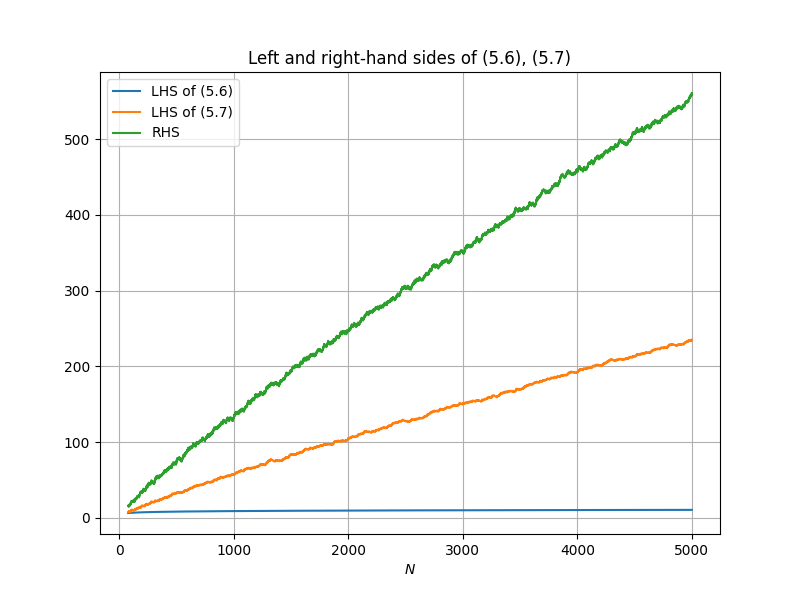
\includegraphics[width=0.8\textwidth]{lhs_rhs.png}
  \caption{A plot of the left and right-hand sides of \eqref{base-test-ineq}, \eqref{test-ineq} for $80 \leq N < 5000$.}\label{fig2}
\end{figure}

\section{The accounting equation}\label{accounting-sec}

Given a $t$-admissible multiset $\tuple$ (which we view as an approximate factorization of $N!$), we can apply the fundamental theorem of arithmetic \eqref{ftoa} to the rational number  $N!/\prod \tuple$ and rearrange to obtain the \emph{accounting equation}
\begin{equation}\label{accounting} 
  \excess_t(\tuple) + \sum_p \nu_p\left( \frac{N!}{\prod \tuple} \right) \log p = \log N! - |\tuple| \log t
\end{equation}
where we define the \emph{$t$-excess} $\excess_t(\tuple)$ of the multiset $\tuple$ by the formula
\begin{equation}\label{excess-def}
  \excess_t(\tuple) \coloneqq \sum_{a \in \tuple} \log \frac{a}{t}.
\end{equation}

\begin{example} Suppose one wishes to factorize $5! = 2^3 \times 3 \times 5$.  The attempted $3$-admissible factorization $\tuple \coloneqq \{3,4,5,5\}$ has a $2$-surplus of $\nu_2(5!/\prod \tuple) = 1$, is in balance at $3$, and has a $5$-deficit of $\nu_5(\prod \tuple/5!) = 1$, so it is not a factorization or subfactorization of $5!$.  The $3$-excess of this multiset is
  $$ \excess_3(\tuple) = \log \frac{3}{3} + \log \frac{4}{3} + \log \frac{5}{3} + \log \frac{5}{3} = 1.3093\dots$$
  and the accounting equation \eqref{accounting} becomes
  $$ 1.3093\dots + \log 2 - \log 5 = 0.3930\dots = \log 5! - 4 \log 3.$$
  If one replaces one of the copies of $5$ in ${\mathcal B}$ with a $2$, this erases both the $2$-surplus and the $5$-deficit, and creates a factorization $\tuple' = \{2,3,4,5\}$ of $5!$; the $3$-excess now drops to
  $$ \excess_3(\tuple) = \log \frac{2}{3} + \log \frac{3}{3} + \log \frac{4}{3} + \log \frac{5}{3}  = 0.3930\dots,$$
  bringing the accounting equation back into balance.
\end{example}
  
In view of \Cref{subfac}, one can now equivalently describe 
$t(N)$ as follows:

\begin{lemma}[Equivalent description of $t(N)$]\label{t-descrip}  $t(N)$ is the largest quantity $t$ for which there exists a $t$-admissible subfactorization of $N!$ with
$$ \excess_t(\tuple) + \sum_p \nu_p\left( \frac{N!}{\prod \tuple} \right) \log p \leq \log N! - N \log t.$$
\end{lemma}

One can view $\log N! - N\log t$ as an available ``budget'' that one can ``spend'' on some combination of $t$-excess and $p$-surpluses.  For $t$ of the form $t = N/e^{1+\delta}$ for some $\delta>0$, the budget can be computed using the Stirling approximation \eqref{stirling} to be $\delta N + O(\log N)$.  The non-negativity of the $t$-excess and $p$-surpluses recovers the trivial upper bound \eqref{trivial}; but note that any prime $p > \frac{t}{\lfloor \sqrt{t} \rfloor}$ must inevitably contribute at least $\log \frac{\lceil t/p\rceil}{t/p}$ to the $t$-excess if it is to appear in the multiset $\tuple$.  By pursuing this line of reasoning, one can obtain an alternate proof of \Cref{upper-crit}; see \cite[Lemma 2.1]{tao}.

\section{Rearranging the standard factorization}\label{rearrange-sec}

In this section we describe an approach to establishing lower bounds on $t(N)$ by starting with the standard factorization $\{1,\dots,N\}$, dividing out some small prime factors from some of the terms, and then redistributing them to other terms.  This approach was introduced in \cite{guy} to give lower bounds of the shape $\frac{t(N)}{N} \geq \frac{3}{16} + o(1)$ (by redistributing powers of two only) and $\frac{t(N)}{N} \geq \frac{1}{4} + o(1)$.  With computer assistance, we are also able to show that $\frac{t(N)}{N} \geq \frac{1}{3}+o(1)$ for sufficiently large $N$, in a simpler fashion than the method used to prove \Cref{main}(iv) in the next section.

\textbf{details needed here}


\section{Modified approximate factorizations}\label{approx-sec}

In this section we present and then analyze an algorithm that starts with an \emph{approximate} factorization $\tuple^{(0)}$ of $N!$, which is $t$-admissible but omits all tiny primes, and is approximately in balance in small and medium primes, and attempts to ``repair'' this factorization to establish a lower bound of the form $t(N) \geq t$.  

To describe the criterion for the algorithm to succeed, it will be convenient to introduce the following notation.
For $a_+,a_- \in [0,+\infty]$, we define the asymmetric norm $|x|_{a_+,a_-}$ of a real number $x$ by the formula
$$ 
|x|_{a_+,a_-} \coloneqq  \begin{cases} 
  a_+ |x| & x\geq 0 \\
  a_- |x| & x\leq 0,
\end{cases}
$$
with the usual convention $+\infty \times 0 = 0$.
If $a_+,a_-$ are finite, this function is Lipschitz with constant $\max(a_+,a_-)$.  One can think of $a_+$ as the ``cost'' of making $x$ positive, and $a_-$ as the
``cost'' of making $x$ negative. 

The analysis of the algorithm is now captured by the following proposition.

\begin{proposition}[Repairing an approximate factorization]\label{repair}  Let $N, K$ be natural numbers, and let $1 \leq t \leq N$ be an additional parameter obeying the conditions
\begin{equation}\label{conditions}
    \frac{t}{K} \geq \sqrt{N}; \quad \frac{t}{K^2} \geq K \geq 5.
\end{equation}
We also assume that there are additional parameters $\kappa_* > 0$ and $0 \leq \gamma_2, \gamma_3 < 1$, such that there exist $3$-smooth numbers
\begin{equation}\label{tlip} 
  t \leq 2^{n_2} 3^{m_2}, 2^{n_3} 3^{m_3} \leq e^{\kappa_*} t
\end{equation}
such that
\begin{equation}\label{nm}
  2m_2 \leq \gamma_2 n_2; \quad n_3 \leq 2\gamma_3 m_3.
\end{equation}
We define the ``norm'' of a pair $n,m$ of real numbers by the formula
$$ \| (n,m) \|_\gamma \coloneqq \max\left( \frac{n-2\gamma_2 m}{1-\gamma_2}, \frac{2m-\gamma_3 n}{1-\gamma_3} \right).$$
Let $\tuple^{(0)}$ be a $t$-admissible multiset of natural numbers, with all elements of $\tuple^{(0)}$ at most $(t/K)^2$, and suppose that one has the inequalities
\begin{equation}\label{delta-cond}
\sum_{i=1}^8 \delta_i \leq \delta
\end{equation}
and
\begin{equation}\label{alpha-cond}
  \sum_{i=1}^7 \alpha_i \leq 1
\end{equation} 
where
\begin{align}
\delta_1 &\coloneqq \frac{1}{N} \excess_t(\tuple^{(1)}) \label{delta1-def}  \\
\delta_2 &\coloneqq \frac{1}{N} \sum_{t/K < p \leq N} f_{N/t}(p/N) \label{delta2-def}  \\
\delta_3 &\coloneqq \frac{\kappa_{4.5}}{N}  \sum_{3 < p_1 \leq t/K} \left|\nu_{p_1}\left( \frac{N!}{\prod \tuple^{(0)}} \right)\right| \label{delta3-def}  \\
\delta_4 &\coloneqq \kappa_{4.5} \sum_{K < p_1 \leq t/K} A_{p_1} \label{delta4-def}  \\
\delta_5 &\coloneqq \kappa_{4.5} \sum_{3 < p_1 \leq K} |A_{p_1} - B_{p_1}|_{\frac{\log p_1}{\log(t/K^2)},1} \label{delta5-def}  \\
\delta_6 &\coloneqq \frac{\kappa_{4.5}}{N} \label{delta6-def}  \\
\delta_7 &\coloneqq \frac{\kappa_*}{\log t} \left( \log \sqrt{12} - B_2 \log 2 - B_3 \log 3\right)\label{delta7-def}  \\
\delta_8 &\coloneqq \frac{2(\log t + \kappa_*)}{N} \label{delta8-def}\\
\delta &\coloneqq \frac{1}{N} \log N! - \log t\label{delta-def}  
\end{align}
\begin{align}
\alpha_1 &\coloneqq \frac{1}{N} \left\| \left( \nu_{2}\left(\prod \tuple^{(0)}\right), \nu_{3}\left(\prod \tuple^{(0)}\right)\right) \right\|_\gamma \label{alpha1-def}  \\
\alpha_2 &\coloneqq \left\| (B_2, B_3) \right\|_\gamma \label{alpha2-def}  \\
\alpha_3 &\coloneqq \frac{\log \frac{t}{K} + \kappa_{**}}{N\log \sqrt{12}} \sum_{3 < p_1 \leq t/K} \left|\nu_{p_1}\left( \frac{N!}{\prod \tuple^{(0)}} \right)\right| \label{alpha3-def}  \\
\alpha_4 &\coloneqq \frac{1}{\log \sqrt{12}} \sum_{K < p_1 \leq t/K} \left(\log \frac{t}{p_1} + \kappa_{**}\right) A_{p_1} \label{alpha4-def}  \\
\alpha_5 &\coloneqq \frac{1}{\log \sqrt{12}} \sum_{3 < p_1 \leq K} \left|A_{p_1} - B_{p_1}\right|_{\frac{\log p_1}{\log(t/K^2)} (\log K^2 + \kappa_{**}), \log p_1 + \kappa_{**}} \label{alpha5-def}  \\
\alpha_6 &\coloneqq \frac{\log t + \kappa_{**}}{N\log \sqrt{12}}  \label{alpha6-def}  \\
\alpha_7 &\coloneqq \max\left( \frac{\log(2N)}{(1-\gamma_2)N\log 2},  \frac{\log(3N)}{(1-\gamma_3)N\log \sqrt{3}}\right)\label{alpha7-def}  
\end{align}
\begin{align}
\kappa_{**} &\coloneqq \max(\kappa^{(2)}_{4.5, \gamma_2}, \kappa^{(3)}_{4.5, \gamma_3}) \label{kappastar-def}  \\
A_{p_1} &\coloneqq \frac{1}{N} \sum_m \nu_{p_1}(m) | \{ a \in \tuple^{(0)}: a = mp \hbox{ for a prime } p > t/K \}| \label{A-def} \\
B_{p_1} &\coloneqq \frac{1}{N} \sum_{m \leq K} \nu_{p_1}(m) \sum_{\frac{t}{m} \leq p < \frac{t}{m-1}} \left \lfloor \frac{N}{p} \right\rfloor,\label{B-def} 
\end{align}
with the convention that the upper bound $p < \frac{t}{m-1}$ in \eqref{B-def} is vacuous when $m=1$.  Then $t(N) \geq t$.
\end{proposition}

In practice, the parameter $K$ will be quite small compared to $N$, and the quantities $\gamma_2, \gamma_3, \kappa_{*}$ will also be somewhat smaller than $1$.

\begin{remark} In the notation of this proposition, \Cref{upper-crit} can essentially be interpreted as a necessary condition $\delta_2 \leq \delta$ for $t(N) \leq t$ to be provable; to use the above proposition effectively, it is thus desirable to have all the other $\delta_i, i \neq 2$ terms be as small as possible.  The criterion in \Cref{t-descrip} can similarly be rewritten as $\delta_1+\delta_9 \leq \delta$, where
  $$ \delta_9 \coloneqq \frac{1}{N} \sum_p \left|\nu_{p_1}\left( \frac{N!}{\prod \tuple^{(0)}} \right)\right|_{\log p, \infty}.$$
In practice, $\delta_9$ is too large (or infinite) for this criterion to be directly useful; the algorithm below is intended to replace this large quantity with something much smaller, and in particular to utilize tiny primes to gain factors such as $\kappa_L$ for various $L$ in the bounds of the main $\delta_i$ terms besides the ``non-negotiable'' $\delta_2$.  The secondary condition \eqref{alpha-cond} can be interpreted as a requirement that ``enough'' tiny primes are available in the factorization of $N!$ to perform such adjustments.
\end{remark}


The rest of this section will be devoted to the proof of this proposition.  It will be convenient to divide the primes into four classes:
  \begin{itemize}
    \item \emph{Tiny primes} $p=2,3$.
    \item \emph{Small primes} $3 < p \leq K$.
    \item \emph{Medium primes} $K < p \leq t/K$.
    \item \emph{Large primes} $p > t/K$.
    \end{itemize}
Initially, the multiset $\tuple^{(0)}$ may have the ``wrong'' number of factors at large primes.  We fix this by applying the following modifications to $\tuple^{(0)}$:
\begin{itemize}
  \item[(a)] Remove all elements of $\tuple^{(0)}$ that are divisible by a large prime $p > t/K$ from the multiset.
  \item[(b)] For each large prime $p > t/K$, add $\nu_p(N!)$ copies of $p \lceil t/p \rceil$ to the multiset.
\end{itemize}
We let $\tuple^{(1)}$ be the multiset formed after completing both Step (a) and Step (b).  We make two simple observations:
\begin{itemize}
\item[(A)] Since the elements of $\tuple^{(0)}$ are at most $(t/K)^2$, all the elements removed in Step (a) are of the form $mp$ where $m \leq t/K$.
\item[(B)] For each large prime $p$ considered in Step (b),  one has $\nu_p(N!) = \lfloor N/p \rfloor$ by \eqref{legendre} and \eqref{conditions}, while $\lceil t/p \rceil \leq K \leq t/K$ (again by \eqref{conditions}).  
\end{itemize}
From this, we see that $\tuple^{(1)}$ is automatically $t$-admissible, and in balance at any large prime $p > t/K$:
$$ \nu_p\left(\frac{N!}{\prod \tuple^{(1)}}\right) = 0.$$
For medium primes $K < p_1 \leq t/K$, one can have some increase in the $p_1$-surplus coming from Step (a), which is described by \eqref{A-def}:
$$ \nu_{p_1}\left(\frac{N!}{\prod \tuple^{(1)}}\right) = \nu_{p_1}\left(\frac{N!}{\prod \tuple^{(0)}}\right) + NA_{p_1}.$$
For small or tiny primes $p \leq K$, one also has some possible decrease in the $p_1$-surplus coming from Step (b), which is described by \eqref{B-def}:
$$ \nu_{p_1}\left(\frac{N!}{\prod \tuple^{(1)}}\right) = \nu_{p_1}\left(\frac{N!}{\prod \tuple^{(0)}}\right) + N(A_{p_1} - B_{p_1}).$$
In particular, we have from \eqref{alpha1-def}, \eqref{alpha2-def} and the triangle inequality that
\begin{equation}\label{alpha-1}
\frac{1}{N} \left\|\left( \nu_2\left(\prod \tuple^{(1)}\right), \nu_3\left(\prod \tuple^{(1)}\right)\right)\right\|_\gamma \leq \alpha_1 + \alpha_2.
\end{equation}

Each element removed in Step (a) reduces the $t$-excess, while each element $p \lceil t/p \rceil$ added in Step (b) increases the $t$-excess by $\log \frac{\lceil t/p \rceil}{t/p}$, so each large prime $t/K < p \leq N$ contributes a net of $\lfloor \frac{N}{p} \rfloor \log \frac{\lceil t/p \rceil}{t/p} = f_{N/t}(p/N)$ to the $t$-excess.  Thus by \eqref{delta1-def}, \eqref{delta2-def} we have
\begin{equation}\label{excess-1} 
  \frac{1}{N} \excess_t(\tuple^{(1)}) \leq \delta_1 + \delta_2.
\end{equation}

Now we bring the multiset $\tuple^{(1)}$ into balance at small and medium primes $3 < p \leq t/K$.  We make the following observations:
\begin{itemize}
\item[(C)]  If an element in $\tuple^{(1)}$ is divisible by some small or medium prime $3 < p \leq t/K$, and one replaces $p$ by $\lceil p \rceil^{\langle 2,3 \rangle}_{4.5}$ in the factorization of that element, then the $p$-deficit decreases by one, while (by \Cref{power-lemma}) the $t$-excess increases by at most $\kappa_{4.5}$, and the quantity $\| (\nu_2(\prod \tuple^{(1)}),\nu_3(\prod \tuple^{(1)}))\|_\gamma$ increases by at most $\frac{\log p + \kappa_{**}}{\log \sqrt{12}}$.  All other $p_1$-surpluses or $p_1$-deficits for $p_1 \neq 2,3,p$ remain unaffected.
\item[(D)]  If one adds an element of the form $m \lceil t/m \rceil^{\langle 2,3 \rangle}_{4.5}$ to $\tuple^{(1)}$ for some $m \leq t/K$ that is the product of small or medium primes $3 < p \leq t/K$, then the $p$-surpluses at small or medium primes $p$ decrease by $\nu_p(m)$, while (by \Cref{power-lemma}) the $t$-excess increases by at most $\kappa_{4.5}$, and the quantity $\| (\nu_2(\frac{N!}{\prod \tuple^{(1)}}), \nu_3(\frac{N!}{\prod \tuple^{(1)}}))\|_\gamma$ increases by at most $\frac{\log(t/m) + \kappa_{**}}{\log \sqrt{12}}$.  The $p$-surpluses or $p$-deficits at medium or large primes remain unaffected.
\end{itemize}

With these observations in mind, we perform the following modifications to the multiset $\tuple^{(1)}$.
\begin{itemize}
\item[(c)] If there is a $p_1$-deficit $\nu_{p_1}(\prod \tuple^{(1)}/N!) > 0$ at some small or medium prime $3 < p_1 \leq t/K$, then we perform the replacement of $p_1$ in one of the elements of $\tuple^{(1)}$ with $\lceil p_1 \rceil^{\langle 2,3\rangle}_{4.5}$ as per observation (C), repeated $\nu_{p_1}(\prod \tuple^{(1)}/N!)$ times, in order to eliminate all such deficits.
\item[(d)] If there is a $p$-surplus $\nu_p(\prod N!/\tuple^{(1)}) > 0$ at some medium prime $K < p \leq t/K$, we add the element 
$p \lceil t/p \rceil^{\langle 2,3 \rangle}_{4.5}$ to $\tuple^{(1)}$ as per observation (D), $\nu_p(\prod N!/\tuple^{(1)})$ times, in order to eliminate all such surpluses at medium primes.
\item[(d')] If there are $p$-surpluses $\nu_p(\prod N!/\tuple^{(1)}) > 0$ at some small primes $3 < p \leq K$, we multiply all these primes together, then apply the greedy algorithm to factor them into products $m$ in the range $t/K^2 < m \leq t/K$, plus at most one exceptional product in the range $1 < m \leq t/K$.  For each of these $m$, add $m \lceil t/m \rceil^{\langle 2,3 \rangle}_{4.5}$ to $\tuple^{(1)}$ as per observation (D), to eliminate all such surpluses at small primes.
\end{itemize}
Call the multiset formed from $\tuple^{(1)}$ formed as the outcome of applying Steps (c), (d), (d') as $\tuple^{(2)}$.  The product of all the primes arising in Step (d') has logarithm equal to
$$ \sum_{3 < p_1 \leq K} \left|\nu_{p_1}\left( \frac{N!}{\prod \tuple^{(1)}} \right) \right|_{\log p_1,0} = \sum_{3 < p_1 \leq K} \left|\nu_p\left( \frac{N!}{\prod \tuple^{(0)}} \right) \right|_{\log p_1,0}$$
and hence the number of non-exceptional $m$ arising in (d') is at most
$$ \sum_{3 < p_1 \leq K} \left|\nu_p\left( \frac{N!}{\prod \tuple^{(0)}} \right) \right|_{\frac{\log p_1}{\log(t/K^2)},0}.$$
The total excess of $\tuple^{(2)}$ is increased in Step (c) by at most
$$ \kappa_{4.5} \sum_{3 < p_1 \leq t/K} \left|\nu_{p_1}\left( \frac{N!}{\prod \tuple^{(1)}} \right) \right|_{0,1}
=  \kappa_{4.5} \sum_{3 < p_1 \leq t/K} \left|\nu_{p_1}\left( \frac{N!}{\prod \tuple^{(0)}} \right) + N(A_{p_1} - B_{p_1}) \right|_{0,1},$$
in Step (d) by at most
$$ \kappa_{4.5} \sum_{K < p_1 \leq t/K} \left|\nu_{p_1}\left( \frac{N!}{\prod \tuple^{(1)}} \right) \right|_{1,0}
=  \kappa_{4.5} \sum_{K < p_1 \leq t/K} \left|\nu_{p_1}\left( \frac{N!}{\prod \tuple^{(0)}} \right) + NA_{p_1} \right|_{1,0},$$
and in Step (c) by at most
$$ \kappa_{4.5} \left(1 + \sum_{3 < p_1 \leq K} \left|\nu_{p_1}\left( \frac{N!}{\prod \tuple^{(0)}} \right) \right|_{\frac{\log p_1}{\log(t/K^2)},0}\right).$$
From the triangle inequality and \eqref{excess-1}, \eqref{delta3-def}, \eqref{delta4-def}, \eqref{delta5-def}, \eqref{delta6-def}, we then have
\begin{equation}\label{excess-2}
   \frac{1}{N} \excess_t(\tuple^{(2)}) \leq \sum_{i=1}^6 \delta_i.
\end{equation}
Similarly, the quantity $\frac{1}{N} \| (\nu_2(\prod \tuple^{(1)}),\nu_3(\prod \tuple^{(1)}))\|_\gamma$ is increased in Step (c) by at most
$$\frac{1}{N\log \sqrt{12}} \sum_{3 < p_1 \leq t/K} \left|\nu_{p_1}\left( \frac{N!}{\prod \tuple^{(0)}} \right) + N(A_{p_1} - B_{p_1}) \right|_{0,\log p_1 + \kappa_{**}},$$
in Step (d) by at most
$$\frac{1}{N\log \sqrt{12}} \sum_{K < p_1 \leq t/K} \left|\nu_{p_1}\left( \frac{N!}{\prod \tuple^{(0)}} \right) + NA_{p_1} \right|_{\log(t/p_1) + \kappa_{**},0},$$
and in Step (d') by at most the sum of
$$\frac{1}{N\log \sqrt{12}} \sum_{3 < p_1 \leq K} \left|\nu_{p_1}\left( \frac{N!}{\prod \tuple^{(0)}} \right) + N(A_{p_1}-B_{p_1}) \right|_{\log(K^2) + \kappa_{**},0}$$
and
$$\frac{1}{N\log \sqrt{12}} \left( \log t + \kappa_{**} \right)$$
so by \eqref{alpha-1}, \eqref{alpha3-def}, \eqref{alpha4-def}, \eqref{alpha5-def}, \eqref{alpha6-def}, and the triangle inequality we have
\begin{equation}\label{alpha-2} 
\frac{1}{N} \| (\nu_2(\prod \tuple^{(2)}), \nu_3(\prod \tuple^{(3)})) \|_\gamma \leq \sum_{i=1}^6 \alpha_i.
\end{equation}

By construction, the multiset $\tuple^{(2)}$ is $t$-admissible, and in balance at all small, medium, and large primes $p > 3$; thus $N!/\prod \tuple^{(2)} = 2^n 3^m$ for some integers $n,m$.  From \eqref{alpha-2}, \eqref{alpha-cond}, \eqref{legendre}, \eqref{alpha7-def} we have
\begin{align*}
n - 2\gamma_2 m &= \nu_2(N!) - 2\gamma_2 \nu_3(N!) - \left(\nu_2\left(\prod \tuple^{(2)}\right) - 2\gamma_2 \nu_3\left(\prod \tuple^{(2)}\right)\right) \\
&\geq \nu_2(N!) - 2\gamma_2 \nu_3(N!) - N (1-\gamma_2) \sum_{i=1}^6 \alpha_i \\
&> N - 
 \frac{\log N}{\log 2} - 1 - \gamma_2 N - N (1-\gamma_2) (1 - \alpha_7) \\
&= N (1-\gamma_2) \alpha_7 - \frac{\log(2N)}{\log 2} \\
&\geq 0
\end{align*}
and similarly
\begin{align*}
  2m - \gamma_3 n &= 2\nu_3(N!) - \gamma_3 \nu_2(N!) - \left(2\nu_3\left(\prod \tuple^{(2)}\right) - \gamma_3 \nu_2\left(\prod \tuple^{(2)}\right)\right) \\
&\geq 2\nu_3(N!) - \gamma_3 \nu_2(N!) - N (1-\gamma_3) \sum_{i=1}^6 \alpha_i \\
&> N - \frac{\log N}{\log \sqrt{3}} - 2 - \gamma_3 N - N (1-\gamma_3) (1 - \alpha_7) \\ 
&= N (1-\gamma_3) \alpha_7 - \frac{\log(3N)}{\log \sqrt{3}} \\
&\geq 0.
\end{align*}
From \eqref{nm} and Cramer's rule we conclude that that $(n,2m)$ lies in the non-negative linear span of $(n_2, 2m_2)$, $(n_3, 2m_3)$, thus
\begin{equation}\label{comb}  (n,2m) = \beta_2 (n_2,2m_2) + \beta_3 (n_3,2m_3)\end{equation}
for some reals $\beta_2,\beta_3 \geq 0$.
We now create the multiset $\tuple^{(3)}$ by adding $\lfloor \beta_2 \rfloor$ copies of $2^{n_2} 3^{m_2}$ and $\lfloor \beta_3 \rfloor$ copies of $2^{n_3} 3^{m_3}$ to $\tuple^{(2)}$.  By \eqref{tlip}, this multiset remains $t$-admissible, and each element added increases the $t$-excess by at most $\kappa_*$.  The number of such elements can be upper bounded using \eqref{comb}, \eqref{legendre} as
\begin{align*}
  \lfloor \beta_2 \rfloor + \lfloor \beta_3 \rfloor &\leq \beta_2 + \beta_3 \\
  &\leq \frac{1}{\log t} \left( \beta_2 (n_2 \log 2 + m_2 \log 3) + \beta_3 (n_3 \log 2 + m_3 \log 3) \right) \\
  &= \frac{1}{\log t} (n \log 2 + m \log 3) \\
  &\leq \frac{1}{\log t} ((\nu_2(N!)-NB_2) \log 2 + (\nu_3(N!)-NB_3) \log 3) \\
  &\leq \frac{1}{\log t} \left(N \log 2 + \frac{N}{2} \log 3 - NB_2 \log 2 - NB_3 \log 3\right) \\
  &= \frac{N \log \sqrt{12}}{\log t} - \frac{N(B_2 \log 2 + B_3 \log 3)}{\log t}.
\end{align*}
By \eqref{excess-2}, \eqref{delta7-def}, we thus have
\begin{equation}\label{excess-3}
 \frac{1}{N} \excess_t(\tuple^{(3)}) \leq \sum_{i=1}^7 \delta_i.
\end{equation}
Meanwhile by construction we see that $\tuple^{(3)}$ is a subfactorization of $N!$ that is in balance at all non-tiny primes, with tiny prime surpluses bounded by
$$ \nu_2\left( \frac{N!}{\prod \tuple^{(3)}}\right) \leq n_2+n_3; \quad \nu_3\left( \frac{N!}{\prod \tuple^{(3)}}\right) \leq m_2+m_3.$$
and thus by \eqref{tlip}, \eqref{delta8-def}, we thus have
$$ \frac{1}{N} \sum_p \nu_p\left( \frac{N!}{\prod \tuple^{(3)}}\right) \log p \leq \frac{\log 2^{n_2} 3^{m_2} + \log 2^{n_3} 3^{m_3}}{N} \leq \delta_8$$
and thus by \eqref{excess-3}, \eqref{delta-cond} we have
$$ \excess_t(\tuple^{(3)}) + \sum_p \nu_p\left( \frac{N!}{\prod \tuple^{(3)}}\right) \log p \leq \log N! - N \log t.$$
Applying \Cref{t-descrip}, we conclude that $t(N) \geq t$ as claimed.

\section{Estimating terms}\label{construction-sec}

In order to use \Cref{repair} for a given choice of $N,t$, we need to find a $t$-admissible multiset $\tuple^{(0)}$ and parameters $K, \kappa_*, \gamma_2, \gamma_3$ obeying \eqref{conditions} as well as good upper bounds on the quantities $\delta_i$, $i=1,\dots,8$ and $\alpha_i$, $i=1,\dots,7$, that can either be evaluated asymptotically or numerically.  Many of these terms will be straightforward to estimate; we discuss only the more difficult ones here.

We introduce a further natural number parameter $A$ and define 
\begin{equation}\label{sigma-def}
  \sigma \coloneqq \frac{3N}{At}.
\end{equation}
We let $\tuple^{(0)}$ be the multiset of $3$-rough elements of the interval $(t, t(1+\sigma)]$, with each element repeated precisely $A$ times.  This is clearly $t$-admissible.  It has no presence at tiny primes, so
\begin{equation}\label{alpha1-vanish}
  \alpha_1 = 0.
\end{equation}
We will also introduce an auxiliary parameter $L$ to assist us with the estimates.  The influence of the parameters $A,K,L$ on the other parameters $\delta_i, \alpha_i$ (and $\gamma_2,\gamma_3,\kappa_{**}$) can be roughly summarized as follows:
\begin{itemize}
\item $\gamma_2, \gamma_3 \asymp \log L / \log N$; assuming this quantity is small enough, we have $\kappa_{**} \asymp 1$.
\item $\delta_1 \asymp 1/A$.
\item $\delta_2 \asymp 1/\log N$.
\item $\delta_3 \asymp A/K\log N$ and $\alpha_3 \asymp A/K$.
\item $\delta_5 \asymp \log^{O(1)} K/\log^2 N$ and $\alpha_2, \alpha_5 \asymp \log^{O(1)} K / \log N$.
\item $\delta_7 \asymp \kappa_L/\log N$.
\item $\delta_4, \delta_6, \delta_8, \alpha_4, \alpha_6, \alpha_7$ will be lower order terms.
\end{itemize}
We will quantify these relationships more precisely below, but they already suggest that one should take $A$ to only be moderately large (e.g., of logarithmic size), that $K$ should only be slightly larger than $A$, and that $L$ should be significantly smaller than $N$.

We use the notation $\sum^*$ to denote summation restricted to $3$-rough numbers, thus for instance $\sum_{a < k \leq b}^* 1$ denotes the number of $3$-rough numbers in $(a,b]$.  We have a simple estimate for such counts:

\begin{lemma}\label{lit}  For any interval $(a,b]$ with $0 \leq a \leq b$ one has $\sum_{a < k \leq b}^* 1 = \frac{b-a}{3} + O_{\leq}(4/3)$.
\end{lemma}

\begin{figure}
  \centering
  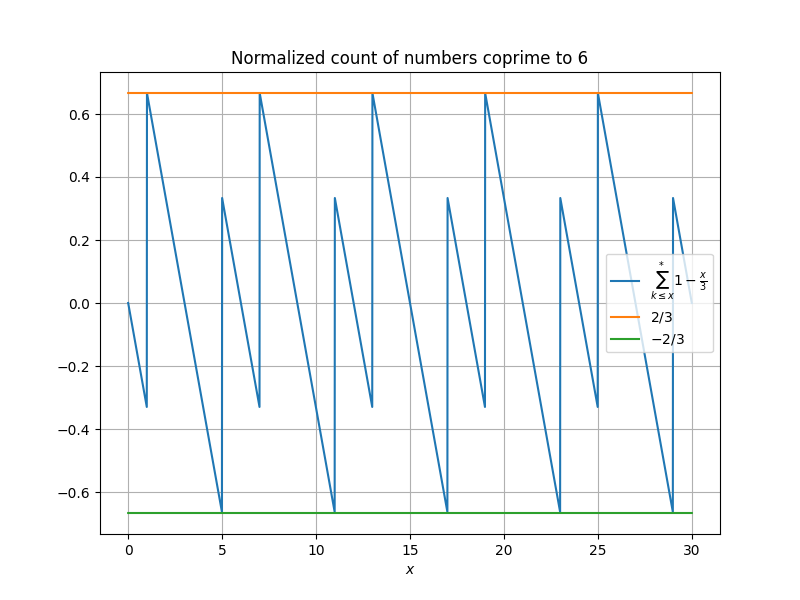
\includegraphics[width=0.8\textwidth]{sawtooth.png}
  \caption{The function $\sum_{k \leq x}^* 1 - \frac{x}{3}$.}\label{fig-saw}
\end{figure}

\begin{proof}  By the triangle inequality, it suffices to show that $\sum_{0 < k \leq x}^* 1 - \frac{x}{3} = O_{\leq}(2/3)$ for all $x \geq 0$.  This is easily verified for $0 \leq x \leq 6$, and the left-hand side is $6$-periodic in $x$, giving the claim; see \Cref{fig-saw}.
\end{proof}

This lets us estimate $\delta_1$:

\begin{lemma}\label{delta1-bound} We have
$$ \delta_1 \leq \frac{3N}{2tA} + \frac{4}{N}.$$
\end{lemma}

\begin{proof}  By definition, we have
$$ \excess_t(\tuple^{(1)}) = A \sum^*_{t < n \leq t(1+\sigma)} \log \frac{n}{t}.$$
By the fundamental theorem of calculus, this is
$$ A \int_0^{t\sigma} \sum^*_{t < n \leq t+h} 1\ \frac{dh}{t+h}.$$
Bounding $\frac{1}{t+h}$ by $\frac{1}{t}$ and applying \Cref{lit}, \eqref{sigma-def}, we conclude that
$$
 \excess_t(\tuple^{(1)}) \leq A \int_0^{3N/A} \left(\frac{h}{3} + \frac{4}{3}\right) \frac{dh}{t} = \frac{3N^2}{2tA} + 4.
$$
and the claim follows.
\end{proof}

To construct $\gamma_2, \gamma_3, \kappa_*, n_2, m_2, n_3, m_3$, we introduce another parameter $L \geq 1$ and assume that
\begin{equation}\label{t-lower}
  t > 3L.
\end{equation}
We define $n_2,n_3,m_2,n_3$ by setting
$$
2^{n_2} 3^{m_2} \coloneqq 2^{n_0} \lceil t/2^{n_0} \rceil^{\langle 2,3 \rangle}; \quad 
2^{n_3} 3^{m_3} \coloneqq 3^{m_0} \lceil t/3^{m_0} \rceil^{\langle 2,3 \rangle}$$
where $2^{n_0}, 3^{m_0}$ are the largest powers of $2,3$ respectively that are at most $t/L$.  By construction and \eqref{kappa-def}, \eqref{tlip} holds with
\begin{equation}\label{kappas-eq}
  \kappa_* = \kappa_L.
\end{equation}
We have
$$  2m_2 \leq \frac{\log \lceil t/2^{n_0} \rceil^{\langle 2,3 \rangle}}{\log \sqrt{3}}  \leq \frac{\log(2L) + \kappa_L}{\log \sqrt{3}}  
$$
and
$$n_2 \geq n_0 \geq \frac{\log t - \log(2L)}{\log 2};$$
similarly
$$ n_3 \leq \frac{\log(3L)+\kappa_L}{\log 2}$$
and
$$ 2m_3 \geq \frac{\log t - \log(3L)}{\log \sqrt{3}}.$$
We conclude that \eqref{nm} holds with
\begin{equation}\label{gammas-def}
\begin{split}
\gamma_2 &\coloneqq \frac{\log 2}{\log \sqrt{3}} \frac{\log(2L) + \kappa_L}{\log t - \log(2L)} \\
\gamma_3 &\coloneqq \frac{\log \sqrt{3}}{\log 2} \frac{\log(3L) + \kappa_L}{\log t - \log(3L)};
\end{split}
\end{equation}
one can of course also take larger values of $\gamma_2,\gamma_3$ if desired.
This lets us compute the quantity $\kappa_{**}$ defined in \eqref{kappastar-def}.

To estimate $\delta_3, \alpha_3$ we use

\begin{lemma}\label{val-bound} For every $3 < p \leq t/K$, one has
\begin{equation}\label{nup} 
  \nu_p\left(\frac{N!}{\prod \tuple^{(1)}}\right) =  
O_{\leq}\left(\frac{4A+3}{3} \left\lceil \frac{\log N}{\log p}  \right\rceil\right).
\end{equation}
\end{lemma}

\begin{proof}
One has
  \begin{align*}
    \nu_p(\prod \tuple^{(1)}) &= A \sum_{t < n \leq t(1+\sigma)}^* \nu_p(n) \\
    &= A \sum_{1 \leq j \leq \frac{\log N}{\log p}} \sum_{t/p^j < n \leq t(1+\sigma)/p^j}^* 1 \\
    &= A \sum_{1 \leq j \leq \frac{\log N}{\log p}} \left(\frac{N}{p^j A} + O_{\leq}(4/3)\right) \\
    &= \frac{N}{p-1} - O_{\leq}^+\left(\frac{1}{p-1}\right)
    + O_{\leq}\left(\frac{4A}{3} \left\lceil \frac{\log N}{\log p}  \right\rceil\right) \\
    &= \frac{N}{p-1} 
    - O_{\leq}^+\left(\left\lceil \frac{\log N}{\log p}  \right\rceil\right)
    + O_{\leq}\left(\frac{4A}{3} \left\lceil \frac{\log N}{\log p}  \right\rceil\right).
  \end{align*}
  Meanwhile, from \eqref{legendre} one has
  $$ \nu_p(N!) = \frac{N}{p-1} - O_{\leq}^+\left(\left\lceil \frac{\log N}{\log p}  \right\rceil\right)$$
and the claim follows.  
\end{proof}

\begin{corollary}\label{delta3-alpha3-bound} One has
$$ \delta_3 \leq \frac{(4A+3)\kappa_{4.5}}{3N} \left(\pi\left(\frac{t}{K} \right) + \frac{\log N}{\log 5} \pi\left(\sqrt{N}\right)\right)$$
and
$$ \alpha_3 \leq \frac{(4A+3) \left(\log \frac{t}{K} + \kappa_{**}\right)}{3N\log \sqrt{12}}  \left(\pi\left(\frac{t}{K} \right) + \frac{\log N}{\log 5} \pi\left(\sqrt{N}\right)\right).$$
\end{corollary}

\begin{proof} This is immediate from \Cref{val-bound} and \eqref{alpha3-def}, \eqref{delta3-def} after noting that $\lfloor \frac{\log N}{\log p} \rfloor \leq 1 + \frac{\log N}{\log 5} 1_{p \leq \sqrt{N}}$ for $3 < p \leq t/K$.
\end{proof}

The main quantities left to estimate are the quantities $\delta_4, \delta_5, \alpha_4, \alpha_5$ that involve $A_{p_1}$.  By construction of $\tuple^{(0)}$, we have
$$
A_{p_1} = \frac{1}{N} \sum_m^* \nu_{p_1}(m) \sum_{\frac{t}{K}, \frac{t}{m} < p \leq \frac{t(1+\sigma)}{m}} A.
$$
In particular, for $p > K(1+\sigma)$ the quantity $A_{p_1}$ vanishes entirely:
\begin{equation}\label{ap1-vanish}
  A_{p_1} = 0.
\end{equation}
For the remaining primes $3 < p \leq K(1+\sigma)$ one has
\begin{equation}\label{ap1-small}
A_{p_1} = \frac{A}{N} \sum_{m \leq K(1+\sigma)}^* \nu_{p_1}(m) \left( \pi\left(\frac{t(1+\sigma)}{m}\right) - \pi\left(\frac{t}{\min(m,K)} \right) \right).
\end{equation}
In practice, these expressions can be adequately controlled by \Cref{osc-lemma}, as can the quantities $B_{p_1}$.

\section{The asymptotic regime}

With the above estimates, we can now establish the lower bound in \Cref{main}(iv).  Thus we aim to show that $t(N) \geq t$ for sufficiently large $N$, where
\begin{equation}\label{main-lower}
   t \coloneqq \frac{N}{e} - \frac{c_0 N}{\log N} + \frac{N}{\log^{1+c_1} N} \asymp N
\end{equation}
and $0 < c_1 < 1$ is a small absolute constant. We use the construction of the previous section with the parameters
\begin{align}
  A &\coloneqq \lfloor \log^2 N \rfloor\label{a-asym}\\
K &\coloneqq \lfloor \log^3 N \rfloor \label{k-asym} \\
L &\coloneqq N^{0.1},\label{l-asym}
\end{align}
so from \eqref{sigma-def} one has
\begin{equation}\label{sigma-alt}
   \sigma = \frac{3N}{tA} \asymp \frac{1}{A} \asymp \frac{1}{\log^2 N}.
\end{equation}
The conditions \eqref{conditions}, \eqref{t-lower} are easily verified for $N$ large enough.

By \eqref{kappas-eq}, \eqref{l-asym}, and \Cref{power-lemma}(ii) we have
$$ \kappa_* \ll \log^{-c} N$$
for some absolute constant $c>0$.  From \eqref{gammas-def}, \eqref{main-lower}, \eqref{l-asym} we have
$$ \gamma_2 = \frac{1}{10} \frac{\log 2}{\log \sqrt{3}} + O\left(\frac{1}{\log N}\right), \quad
 \gamma_3 = \frac{1}{10} \frac{\log \sqrt{3}}{\log 2} + O\left(\frac{1}{\log N}\right)
$$
and hence by \eqref{kappastar-def},  \eqref{kappastar-2-def}, \eqref{kappastar-3-def} we have for sufficiently large $N$ that
$$ \kappa_{**} \ll 1.$$
By \Cref{repair}, it thus suffices to establish the inequalities \eqref{delta-cond}, \eqref{alpha-cond}.
Several of the quantities $\delta, \delta_i, \alpha_i$ can now be immediately estimated using \eqref{alpha1-vanish}, \eqref{delta1-bound}, \Cref{delta3-alpha3-bound}, \eqref{stirling}, and the prime number theorem:
\begin{align*}
  \delta_1 &\ll \frac{1}{A} \asymp \frac{1}{\log^2 N} \\
  \delta_3 &\ll \frac{A}{K \log N} \asymp \frac{1}{\log^2 N} \\
  \delta_6 &\ll \frac{1}{N} \\
  \delta_7 &\ll \frac{\kappa_*}{\log N} \ll \frac{1}{\log^{1+c} N} \\
  \delta_8 &\ll \frac{\log N}{N} \\
  \delta &= \frac{ec_0}{\log N} + \frac{e}{\log^{1+c_1} N} + O\left( \frac{1}{\log^2 N} \right)\\  
\end{align*}
\begin{align*}
  \alpha_1 &= 0 \\
  \alpha_3 &\ll \frac{A}{K} \asymp \frac{1}{\log N} \\
  \alpha_6, \alpha_7 &\ll \frac{\log N}{N} \\
\end{align*}
On the interval $(t/NK,1]$, the function $f_{N/t}$ is piecewise monotone with $O(K)$ pieces, and bounded by $1$, so its augmented total variation norm is $O(K)$.  Applying \eqref{delta2-def} and \Cref{osc-lemma} (with classical error term), we have
\begin{align*}
\delta_2 &\leq \frac{1}{\log(t/K)} \int_{t/NK}^1 f_{N/t}(x)\ dx + O\left( \frac{1}{\log^2 N} \right) \\
&\leq \frac{1}{\log N} \int_{1/eK}^{N/et} f_{N/t}(etx/N)\ dx + O\left( \frac{1}{\log^2 N} \right)
\end{align*}
where we have used \eqref{falpha-bound} to manage error terms.
Similarly to the proof of \Cref{upper-bound}, the function $f_{N/t}(etx/N)$ differs from $f_e(x)$ outside of an exceptional set of measure $O(1/\log N)$, and hence by \eqref{c0-def} (and \eqref{falpha-bound}) we have
$$ \delta_2 \leq \frac{ec_0}{\log N} + O\left( \frac{1}{\log^2 N} \right).$$
To finish the verification of the conditions \eqref{delta-cond}, \eqref{alpha-cond}, it will suffice to show that
\begin{equation}\label{delta-remaining}
\delta_4, \delta_5 \ll \frac{(\log\log N)^{O(1)}}{\log^2 N}
\end{equation}
and
\begin{equation}\label{alpha-remaining}
\alpha_2, \alpha_4, \alpha_5 \ll \frac{(\log\log N)^{O(1)}}{\log N}.
\end{equation}
By Mertens' theorem (or \Cref{osc-lemma}) and \eqref{delta4-def}, \eqref{delta5-def}, \eqref{alpha2-def}, \eqref{alpha4-def}, \eqref{alpha5-def}, \eqref{sigma-alt}, it suffices to show that
\begin{equation}\label{ap1-bound}
A_{p_1}, B_{p_1} \ll \frac{(\log\log N)^{O(1)}}{p_1 \log N} 
\end{equation}
for all $p_1 \leq K(1+\sigma)$ (recalling from \eqref{ap1-vanish} that $A_{p_1}$ vanishes for any larger $p_1$), as well as the variant
\begin{equation}\label{ap1-diff}
  |A_{p_1}-B_{p_1}|_{0,1} \ll \frac{(\log\log N)^{O(1)}}{p_1 \log^2 N}
\end{equation}
for $3 < p_1 \leq K$.

For \eqref{ap1-bound} we use \eqref{ap1-small}, \eqref{B-def}, and the crude bound 
\begin{equation}\label{crude}
  \nu_{p_1}(m) \ll 1_{p_1|m} \log\log N
\end{equation}
 for $m \leq K(1+\sigma)$, and reduce to showing that
$$ \frac{A}{N} \sum_{m \leq K(1+\sigma)} 1_{p_1|m} \left( \pi\left(\frac{t(1+\sigma)}{m}\right) - \pi\left(\frac{t}{\min(m,K)} \right) \right).
\ll \frac{(\log\log N)^{O(1)}}{p_1 \log N}$$
and
$$ \frac{1}{N} \sum_{m \leq K} 1_{p_1|m} \sum_{\frac{t}{m} \leq p < \frac{t}{m-1}} \left \lfloor \frac{N}{p} \right\rfloor \ll
\frac{(\log\log N)^{O(1)}}{p_1 \log N}.$$ 
But from the Brun--Titchmarsh inequality (or \Cref{osc-lemma}) and \eqref{sigma-alt} one has
$$ \pi\left(\frac{t(1+\sigma)}{m}\right) - \pi\left(\frac{t}{\min(m,K)}\right) \ll \frac{t\sigma}{m \log N} \ll \frac{N}{Am \log N}$$
and
$$ \sum_{\frac{t}{m} \leq p < \frac{t}{m-1}} \left \lfloor \frac{N}{p} \right\rfloor \ll \frac{tm}{m^2 \log N} \ll \frac{N}{m \log N}$$
and the claim then follows from summing the harmonic series.

It remains to show \eqref{ap1-diff}.  For $3 < p_1 \leq K$, we see from \eqref{ap1-small}, \eqref{sigma-alt}, \eqref{crude} and \Cref{osc-lemma} (with classical error term) that
\begin{align*}
A_{p_1} &\geq \frac{1}{N} \sum_{m \leq K(1+\sigma)}^* \nu_{p_1}(m) \left( \frac{A t \sigma}{m \log N} + O\left( \frac{(\log\log N)^{O(1)}A t \sigma}{m \log^2 N} \right) \right) \\
&= \frac{1}{\log N} \sum_{m \leq K(1+\sigma)}^* \nu_{p_1}(m) \frac{3}{m}+ O\left( \frac{(\log\log N)^{O(1)}}{\log^2 N} \right) \\
&= \frac{1}{\log N} \sum_{m \leq K}^* \nu_{p_1}(m) \frac{3}{m}+ O\left( \frac{(\log\log N)^{O(1)}}{\log^2 N} \right) 
\end{align*}
and similarly from \eqref{B-def}, \eqref{crude}, and \Cref{osc-lemma} (again with classical error term) 
\begin{align*}
  B_{p_1} &\leq
  \frac{1}{N} \sum_{m \leq K} \nu_{p_1}(m) \sum_{\frac{t}{m} \leq p < \frac{t}{m-1}} \frac{N}{p}  \\
  &\leq \frac{1}{N} \sum_{m \leq K} \nu_{p_1}(m) \left( \frac{N}{\log(t/m)} \int_{t/m}^{t/(m-1)} \frac{dx}{x} + O\left( \frac{N}{\log^{10} N} \right) \right) \\
  &\leq \frac{1}{\log N} \sum_{m \leq K} \nu_{p_1}(m) \log \frac{m}{m-1} + O\left( \frac{(\log\log N)^{O(1)}}{\log^2 N} \right)
\end{align*}
so it will suffice to establish the inequality
\begin{equation}\label{key-ineq} 
   \sum_{m \leq K} \nu_{p_1}(m) \log \frac{m}{m-1} \leq \sum_{m \leq K}^* \nu_{p_1}(m) \frac{3}{m}
\end{equation}
for all $p_1 > 3$.
  
Writing $\nu_{p_1}(m) = \sum_{j \geq 1} 1_{p_1^j|m}$, it suffices to show that
  $$ \sum_{m \leq K; p^j|m} \frac{3}{m} 1_{(m,6)=1} - \log \frac{m}{m-1} \geq 0.$$
Making the change of variables $m = p_1^j n$, it suffices to show that
  $$ \sum_{n \leq K'} \frac{3}{n} 1_{(n,6)=1} - p_1^j \log \frac{p_1^j n}{p_1^j n - 1} \geq 0$$
  for any $K' > 0$.   Using the bound
  $$ \log \frac{p_1^jn}{p_1^jn - 1} = \int_{p_1^jn-1}^{p_1^jn} \frac{dx}{x} \leq \frac{1}{p_1^jn-1}$$
  and $p^j \geq 5$, we have
  $$ p_1^j \log \frac{p_1^j n}{p_1^j n - 1} \leq \frac{1}{n-0.2}$$
  and so it suffices to show that
  \begin{equation}\label{kb}
  \sum_{n \leq K'}^* \frac{3}{n} 1_{(n,6)=1} - \frac{1}{n-0.2} \geq 0.
  \end{equation}
  Since 
  $$ \sum_{n=1}^\infty \frac{1}{n-0.2}-\frac{1}{n} = \psi(0.8)-\psi(1) = 0.353473\dots,$$
  where $\psi$ here denotes the digamma function rather than the von Mangoldt summatory function, it will suffice to show that
  \begin{equation}\label{kb-2}
  \sum_{n \leq K'} \frac{3}{n} 1_{(n,6)=1} - \frac{1}{n} \geq 0.4.\end{equation}
  This can be numerically verified for $K' \leq 100$, with substantial room to spare for $K'$ large; see \Cref{fig:kb}. On a block $6a-1 \leq n \leq 6a+4$ with $a>1$, the sum is positive:
  \begin{align*}
  \sum_{6a-1 \leq n \leq 6a+4}^* \frac{3}{n}  - \frac{1}{n } &= \left(\frac{1}{6a-1} - \frac{1}{6a}\right) + \left(\frac{1}{6a-1} - \frac{1}{6a+2}\right)\\
  &\quad + \left(\frac{1}{6a+1} - \frac{1}{6a+3}\right) + \left(\frac{1}{6a+1} - \frac{1}{6a+4}\right) \\
  &\quad > 0.
  \end{align*}
The inequality for $K'>100$ is then easily verified from the $K' \leq 100$ data and the triangle inequality.
  
  \begin{figure}
  \centering
  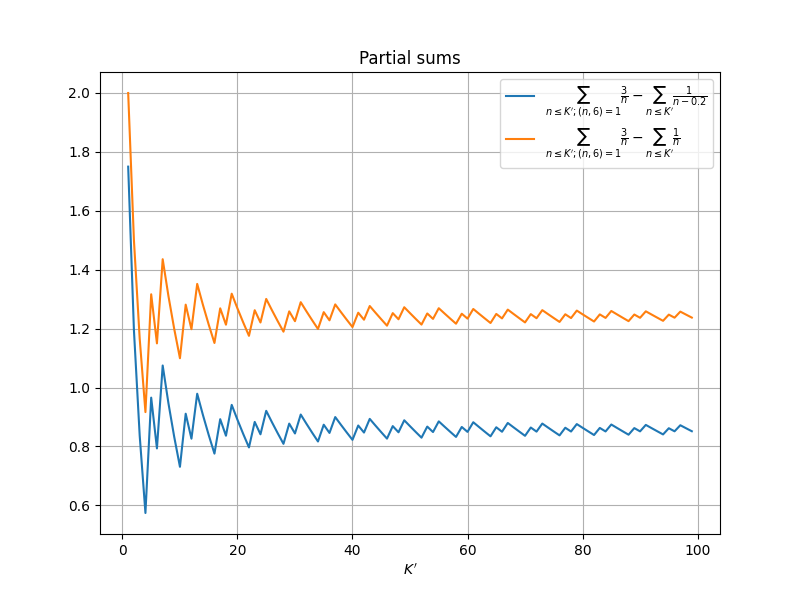
\includegraphics[width=0.5\textwidth]{key_ineq.png}
  \caption{A plot of \eqref{kb}, \eqref{kb-2}.}
  \label{fig:kb}
  \end{figure}







\section{Guy--Selfridge conjecture}

We now establish the Guy--Selfridge conjecture $t(N) \geq N/3$ in the range
$$ N \geq N_0 \coloneqq 10^{11}.$$
We will apply \Cref{repair} with the construction in \Cref{construction-sec} and the choice of parameters
\begin{align*}
  t &\coloneqq N/3\\
  A &\coloneqq 189\\
  K &\coloneqq 293 \\
  L &\coloneqq 4.5;
\end{align*}
the choice of $A$ and $K$ was obtained after some numerical experimentation.  In particular, by \eqref{sigma-def} we have
$$ \sigma = \frac{3N}{At}=\frac{9}{189} =0.047619\dots$$
One can readily check the required conditions \eqref{conditions}, \eqref{t-lower} for $N \geq N_0$, so it remains to verify the hypotheses \eqref{delta-cond}, \eqref{alpha-cond} of \Cref{repair} in this range.  Some of the quantities in these hypotheses involve sums over large ranges, such as $(t/K,N]$; but one can use \Cref{osc-lemma} to obtain adequate upper or lower bounds on such quantities, leaving one with sums over short ranges such as $p \leq K$ or $p \leq K(1+\sigma)$.  As such, all of the bounds needed can be quickly computed even for very large $N$ with simple computer code\footnote{\url{https://github.com/teorth/erdos-guy-selfridge/blob/main/src/python/interval_computations.py}}.

Many of the bounds we will use will be monotone decreasing in $N$, so that they only need to be tested at the left endpoint $N=N_0$.  However, this is not the case for all of the bounds, as some involve subtracting one monotone quantity from another.  For those estimates, we will initially only establish bounds in two extreme cases, $N=N_0$ and $N \geq 10^{70}$, and discuss how to cover the intervening ranges $N_0 < N < 10^{70}$ at the end of the section.
  
We now bound some of the terms appearing in \Cref{repair}. From \Cref{power-lemma} we have
$$ \kappa_{4.5} = \log \frac{4}{3} =0.28768\dots.$$

From \eqref{gammas-def} one can take
$$ \gamma_2 \coloneqq \frac{\log 2}{\log \sqrt{3}} \frac{\log(2L) + \kappa_L}{\log(N_0/3) - \log(2L)} = 0.1423165\dots$$
and
$$\gamma_3 \coloneqq \frac{\log \sqrt{3}}{\log 2} \frac{\log(3L) + \kappa_L}{\log(N_0/3) - \log(3L)} =  0.1059116 \dots$$
for all $N \geq N_0$; by \eqref{kappastar-def} and some calculation we then have
$$ \kappa_{**} \leq 6.830101\dots.$$

From \eqref{stirling} one has
$$ \delta \geq \log N - \log t = \log \frac{3}{e} = 0.0986122\dots$$
for all $N \geq N_0$.  

We will use this lower bound as our unit of reference for all other $\delta_i$ quantities, bounding them by suitable multiples of $\delta$.  For instance, from \eqref{delta1-bound} one has
$$ \delta_1 \leq \frac{9}{2A} + \frac{4}{N_0} \leq 0.241447 \delta$$
for all $N \geq N_0$.

From \eqref{delta2-def} and \Cref{osc-lemma}, and the monotonicity of $E(N)/N$, one has
\begin{align*}
  \delta_2 &\leq \frac{\int_{1/3K}^1 f_3(x)\ dx}{\log(t/K)}  + \frac{\|f_3\|_{\mathrm{TV}((1/3K,1])}}{\log(t/K)}  \frac{E(N)}{N} \\
  &\leq \frac{0.919785}{\log(N_0/3K)}  + \frac{1159.795}{\log(N_0/3K)}  \frac{E(N_0)}{N_0} \\
  &\leq 0.504735 \delta
\end{align*}
for all\footnote{Despite the seemingly large numerator, the second term is in fact negligible in the regime $N \geq N_0$, due to the square root type decay in $E(N)/N$.} $N \geq N_0$.  For $N \geq 10^{70}$ we may replace $N_0$ by $10^{70}$ and obtain the significantly better bound
$$ \delta_2 \leq 0.060410 \delta.$$

From \Cref{delta3-alpha3-bound} and \eqref{pi-upper} one has
\begin{align*}
\delta_3 &\leq \frac{(4A+3)\kappa_{4.5}}{3} \left(
\frac{1}{3K \log \frac{N}{3K}} + \frac{1.2762}{3K \log^2 \frac{N}{3K}}
+ \frac{\log N}{\sqrt{N} \log \sqrt{N}\log 5 } + \frac{1.2762 \log N}{\sqrt{N} \log^2 \sqrt{N}\log 5 } \right) \\
&\leq \frac{(4A+3)\kappa_{4.5}}{3} \left(
  \frac{1}{3K \log\frac{N_0}{3K}} + \frac{1.2762}{3K \log^2\frac{N_0}{3K}}
  + \frac{\log N_0}{\sqrt{N_0} \log \sqrt{N_0}\log 5 } + \frac{1.2762 \log N_0}{\sqrt{N_0} \log^2 \sqrt{N_0}\log 5 } \right) \\
&\leq 0.051574 \delta
\end{align*}
for all $N \geq N_0$.

We skip $\delta_4, \delta_5, \delta_7$ for now.  From \eqref{delta6-def} we have
$$ \delta_6 \leq \frac{\kappa_{4.5}}{N_0} \leq 3 \times 10^{-11} \delta$$
for all $N \geq N_0$, and from \eqref{delta8-def} we have
$$ \delta_8 \leq \frac{2(\log(N_0/3) + \kappa_{4.5})}{N_0} \leq 6 \times 10^{-10} \delta$$
for all $N \geq N_0$, so these two terms are negligible in the analysis.

From \eqref{alpha1-vanish} we have
$$ \alpha_1 = 0.$$
We skip $\alpha_2, \alpha_4, \alpha_5$ for now.  From \Cref{delta3-alpha3-bound} and \eqref{pi-upper} one has
\begin{align*}
  \alpha_3 &\leq \frac{4A+3}{3\log \sqrt{12}} \left(\log \frac{N}{3K} + \kappa_{**}\right)  \\
&\quad \times \left(
  \frac{1}{3K \log\frac{N}{3K}} + \frac{1.2762}{3K \log^2\frac{N}{3K}}
  + \frac{\log N}{\sqrt{N} \log \sqrt{N}\log 5 } + \frac{1.2762 \log N}{\sqrt{N} \log^2 \sqrt{N}\log 5 } \right).
\end{align*}
Expanding out the product, one can check that all terms are non-increasing in $N$; so we may substitute $N_0$ for $N$ in the right-hand side, which after some calculation gives
$$ \alpha_3 \leq 0.361121$$
for all $N \geq N_0$.
From \eqref{alpha6-def} we have
\begin{align*}
   \alpha_6 &\leq \frac{\log(N_0/3) + \kappa_{**}}{N_0 \log \sqrt{12}} \\
   &\leq 3 \times 10^{-10}
\end{align*}
for all $N \geq N_0$, and similarly from \eqref{alpha7-def} we have
\begin{align*}
\alpha_7 &\leq \max\left( \frac{\log(2N_0)}{(1-\gamma_2)N_0\log 2},  \frac{\log(3N_0)}{(1-\gamma_3)N_0\log \sqrt{3}}\right) \\
&\leq 6 \times 10^{-10}
\end{align*}
for all $N \geq N_0$.
so the contribution of these two terms are negligible.

Conveniently\footnote{Even if this were not the case, the quantities $\delta_4,\alpha_4$ should be viewed as lower order terms, and are far smaller than several of the other $\delta_i$ or $\alpha_i$ for typical choices of parameters.}, the choice of parameters $A,K$ ensure that there are no primes in the range
$$ 293 = K < p \leq K(1+\sigma) = K(1+\sigma)=306.952\dots$$
and thus
$$ \delta_4=\alpha_4 = 0$$
for all $N \geq N_0$.

The remaining terms $\delta_5, \delta_7, \alpha_2, \alpha_5$ to estimate involve the quantities $A_{p_1}, B_{p_1}$ defined in \eqref{A-def}, \eqref{B-def}, and require a bit more care.  For $B_{p_1}$, we can split the expression as
$$ B_{p_1} = \sum_{m \leq K} \nu_{p_1}(m) \sum_{k: a_{k,m} < b_{k,m}} \frac{k}{N} (\pi( N b_{k,m} ) - \pi(N a_{k,m}))$$
where 
$$ a_{k,m} \coloneqq \max\left( \frac{1}{3m}-, \frac{1}{k} \right); \quad b_{k,m} \coloneqq \max\left( \frac{1}{3(m-1)}-, \frac{1}{k-1} \right)$$
where the $-$ denotes the subtraction of an infinitesimal quantity to reflect the restriction to the range $\frac{t}{m} \leq p < \frac{t}{m-1}$ rather than
$\frac{t}{m} < p \leq \frac{t}{m-1}$.  Using \Cref{osc-lemma} (and a limiting argument), we can upper bound this quantity by
$$ B_{p_1} \leq \sum_{m \leq K} \nu_{p_1}(m) \sum_{k: a_{k,m} < b_{k,m}} \left(\frac{k}{2\log(N a_{k,m})}+\frac{k}{2\log(N b_{k,m})}\right) (a_{k,m}-b_{k,m}) + 2\frac{E(N b_{k,m})}{N \log(N a_{k,m})} $$
and lower bound it by
\begin{align*}
   B_{p_1} &\geq \sum_{m \leq K} \nu_{p_1}(m) \sum_{k: a_{k,m} < b_{k,m}} \frac{k\left(1-\frac{2}{\sqrt{a_{k,m} N}}\right)}{\log(N (a_{k,m}+b_{k,m})/2)}  (a_{k,m}-b_{k,m}) - 2\frac{E(N b_{k,m})}{N \log(N a_{k,m})}
\end{align*}
We caution here that while the upper bound for $B_{p_1}$ is monotone decreasing in $N$, the lower bound does not have a favorable monotonicity property, particularly as it will be used when \emph{subtracting} copies of $B_{p_1}$ rather than \emph{adding} then.

From the monotonicity of the upper bound, one can use \eqref{alpha2-def} to calculate that 
$$ \alpha_2 \leq 0.269878$$
for all $N \geq N_0$.  For \eqref{delta7-def}, subtraction is involved, and one must proceed with more caution.  For $N=N_0$, one has
$$ \delta_7 \leq 0.11359 \delta.$$
For $N \geq 10^{70}$, we simply discard the negative terms here and obtain the bound
$$ \delta_7 \leq \frac{\kappa_{4.5} \log \sqrt{12}}{\log(10^{70}/3)}  \leq 0.02212 \delta$$

As for the $A_{p_1}$, we know from \eqref{ap1-vanish} that this vanishes unless $3 < p_1 \leq K(1+\sigma)$.  From \eqref{ap1-small} and \Cref{osc-lemma} one has the upper bound
\begin{align*}
A_{p_1} &\leq \sum_{m \leq K(1+\sigma)}^* \left(\frac{A \nu_{p_1}(m)}{2\log(N/3\min(m,K))} + \frac{A \nu_{p_1}(m)}{2\log(N(1+\sigma)/3m)} \right) \left( \frac{1+\sigma}{3m} - \frac{1}{3\min(m,K)}\right) \\
& \quad \quad + \frac{A \nu_{p_1}(m)}{\log(N/3\min(m,K))} \frac{2E(N(1+\sigma)/3m)}{N}  
\end{align*}
and the lower bound
\begin{align*}
A_{p_1} &\geq \sum_{m \leq K(1+\sigma)}^* \frac{A \nu_{p_1}(m)\left(1-\frac{2}{\sqrt{N_0/3\min(m,K)}}\right) }{\log((N/3\min(m,K) + N(1+\sigma)/3m)/2)} \left(\frac{1+\sigma}{3m} - \frac{1}{3\min(m,K)}\right) \\
& \quad \quad - \frac{A \nu_{p_1}(m)}{\log(N/3\min(m,K))}  \frac{2E(N(1+\sigma)/3m)}{N}.
\end{align*}
Again, the upper bound is monotone decreasing in $N$, but the lower bound does not have a favorable monotonicity. At $N=N_0$, one can calculate using these bounds and \eqref{delta5-def}, \eqref{alpha5-def} to obtain
\begin{align*}
\delta_5 &\leq 0.06203 \delta \\
\alpha_5 &\leq 0.31418
\end{align*}
which, when combined with the previous bounds, gives
$$ \sum_{i=1}^8 \delta_i  \leq 0.9740 \delta$$
and 
$$ \sum_{i=1}^7 \alpha_i \leq 0.9452$$
at $N=N_0$, thus verifying \eqref{delta-cond}, \eqref{alpha-cond} in those cases.

For $N \geq 10^{70}$, we use the triangle inequality to crudely upper bound
$$ \delta_5 \leq \kappa_{4.5} \sum_{3 < p_1 \leq K} \frac{\log p_1}{\log(t/K^2)} A_{p_1} + B_{p_1}$$
and
$$ \alpha_5 \leq \frac{1}{\log \sqrt{12}} \sum_{3 < p_1 \leq K}  \frac{(\log K^2+\kappa_{**})\log p_1}{\log(t/K^2)} A_{p_1} + (\log p_1 + \kappa_{**}) B_{p_1}.$$
The bounds available for the right-hand side are now monotone in $N$, and one can calculate that
\begin{align*}
  \delta_5 &\leq 0.077301 \delta \\
  \alpha_5 &\leq 0.184975
  \end{align*}
for $N \geq 10^{70}$. This is better than the previous bound for $\alpha_5$.  For $\delta_5$, the bound is slightly worse, but this is more than compensated for by the improved bounds on $\delta_2$, $\delta_7$, and \eqref{delta-cond}, \eqref{alpha-cond} can be verified here with significant room to spare.

This completes the proof of \Cref{main}(iii) (and hence \Cref{main}(ii)) in the cases $N=N_0$ and $N \geq 10^{70}$.  It remains to cover the intermediate range $N_0 < N \leq 10^{70}$.  Here we adopt the perspective of interval arithmetic.  If $N$ is constrained to a given interval, such as $[10^{11}, 5 \times 10^{11}]$, we can use the worst-case upper and lower bounds for $A_{p_1}, B_{p_1}$ to obtain conservative upper bounds on the most delicate quantities
$\delta_5, \delta_7, \alpha_2, \alpha_5$, thus potentially verifying the conditions \eqref{delta-cond}, \eqref{alpha-cond} simultaneously for all $N$ in such an interval.  As it turns out, there is enough room to spare in these estimates, particularly for large $N$, that this strategy works using only a small number of intervals; specifically, by considering $N$ in the intervals
$$ [10^{11}, 5 \times 10^{11}]; \quad [5 \times 10^{11}, 10^{14}]; \quad [10^14, 10^{20}]; \quad [10^{20}, 10^{70}]$$
one can check that such bounds are sufficient to verify \eqref{delta-cond}, \eqref{alpha-cond} in these cases.  This now verifies \Cref{main}(ii), (iii) for all $N \geq 10^{11}$.
(In fact, with more effort, this verification can be pushed down to $N \geq 6 \times 10^{10}$ using the same choice of parameters $A,K,L$.)
  
\appendix

\section{Distance to the next \texorpdfstring{$3$}{3}-smooth number}\label{power-sec}

We now establish the various claims in \Cref{power-lemma}.  We begin with part (iii).  The claim \eqref{mod-kappa} is immediate from \eqref{kappa-def}, \eqref{fancy-kappa-def}.  Now prove \eqref{12-2}, \eqref{12-3}.  If we write $\lceil x/12^a \rceil^{\langle 2,3 \rangle} = 2^b 3^c$, then by \eqref{kappa-def} we have
$$ b \log 2 + c \log 3 \leq \log x - a \log 12 + \kappa_L,$$
while from definition of $a$ we have
\begin{equation}\label{xa12}
  \log x - a \log 12 \leq \log(12L).
\end{equation}
We now compute
\begin{align*}
  \frac{\nu_2(\lceil x \rceil^{\langle 2,3\rangle}_L) - 2 \gamma \nu_3(\lceil x \rceil^{\langle 2,3\rangle}_L)}{1-\gamma} 
  &= \frac{2a+b - 2\gamma(a+c)}{1-\gamma} \\
  &\leq 2a + \frac{\log x - a \log 12 + \kappa_L}{(1-\gamma) \log 2}  \\
  &= \frac{\log x}{\log \sqrt{12}} + \left( \frac{1}{(1-\gamma)\log 2} - \frac{1}{\log \sqrt{12}}\right) \left(\log x - a \log 12\right)\\
  &\quad 
  + \frac{\kappa_L}{(1-\gamma)\log 2} 
\end{align*}
giving \eqref{12-2} from \eqref{xa12}; similarly, we have
\begin{align*}
  \frac{2\nu_3(\lceil x \rceil^{\langle 2,3\rangle}_L) - \gamma \nu_2(\lceil x \rceil^{\langle 2,3\rangle}_L)}{1-\gamma} 
  &= \frac{2(a+c) - \gamma(2a+b)}{1-\gamma} \\
  &\leq 2a + \frac{2(\log x - a \log 12 + \kappa_L)}{(1-\gamma) \log 3}  \\
  &= \frac{\log x}{\log \sqrt{12}} + \left( \frac{2}{(1-\gamma)\log 3} - \frac{1}{\log \sqrt{12}}\right) \left(\log x - a \log 12\right)\\
  &\quad + \frac{\kappa_L}{(1-\gamma)\log \sqrt{3}} 
\end{align*}
giving \eqref{12-3} from \eqref{xa12}.

To prove parts (i) and (ii) of \Cref{power-lemma}, we establish the following lemma to upper bound $\kappa_L$.

\begin{lemma}\label{lemcount-0}  If $n_1,n_2,m_1,m_2$ are natural numbers such that $n_1+n_2, m_1+m_2 \geq 1$ and
$$ \frac{3^{m_1}}{2^{n_1}}, \frac{2^{n_2}}{3^{m_2}} \geq 1$$
then
$$ \kappa_{\min( 2^{n_1+n_2},3^{m_1+m_2})/6} \leq \log \max\left(\frac{3^{m_1}}{2^{n_1}}, \frac{2^{n_2}}{3^{m_2}}\right).$$
\end{lemma}

\begin{proof}  If $\min( 2^{n_1+n_2},3^{m_1+m_2})/6 \leq t \leq 2^{n_2-1} 3^{m_1-1}$, then we have
\begin{equation}\label{tb} 
  t \leq 2^{n_2-1} 3^{m_1-1} \leq \max\left(\frac{3^{m_1}}{2^{n_1}}, \frac{2^{n_2}}{3^{m_2}}\right) t,
\end{equation}
so we are done in this case.  Now suppose that $t > 2^{n_2-1} 3^{m_1-1}$.
If we write $\lceil t \rceil^{\langle 2,3 \rangle} =2^n 3^m$ be the smallest $3$-smooth number that is at least $t$, then we must have $n \geq n_2$ or $m \geq m_1$ (or both).  Thus at least one of $\frac{2^{n_1}}{3^{m_1}} 2^n 3^m$ and $\frac{3^{m_2}}{3^{n_2}} 2^n 3^m$ is an integer, and is thus at most $t$ by construction.  This gives \eqref{tb}, and the claim follows.
\end{proof}

Some efficient choices of parameters for this lemma are given in \Cref{approx-table}.  For instance, $\kappa_{4.5} \leq \log\frac{4}{3} = 0.28768\dots$ and $\kappa_{40.5} \leq \log \frac{32}{27} = 0.16989\dots$.  In fact, since $\lceil 4.5+\eps \rceil^{\langle 2,3\rangle} = 6$ and $\lceil 40.5+\eps \rceil^{\langle 2,3\rangle} = 48$ for all sufficiently small $\eps>0$, we see that these bounds are sharp (And similarly for the other entries in \Cref{approx-table}); this establishes part (i).

\begin{table}[ht]
\centering
\begin{tabular}{|c|c|c|c|c|c|}
\hline
$n_1$ & $m_1$ & $n_2$ & $m_2$ & $\min(2^{n_1+n_2},3^{m_1+m_2})/6$ & $\log \max(3^{m_1}/2^{n_1}, 2^{n_2}/3^{m_2})$ \\
\hline
$1$ & $1$ & $\mathbf{1}$ & $\mathbf{0}$ & $1/2 = 0.5$ & $\log 2 = 0.69314\dots$ \\
\hline
$\mathbf{1}$ & $\mathbf{1}$ & $2$ & $1$ & $2^2/3 = 1.33\dots$ & $\log (3/2) = 0.40546\dots$\\
\hline
$3$ & $2$ & $\mathbf{2}$ & $\mathbf{1}$ & $3^2/2 = 4.5$ & $\log (2^2/3) = 0.28768\dots$ \\
$3$ & $2$ & $\mathbf{5}$ & $\mathbf{3}$ & $3^4/2 = 40.5$ & $\log (2^5/3^3) = 0.16989\dots$ \\
\hline
$\mathbf{3}$ & $\mathbf{2}$ & $8$ & $5$ & $2^{10}/3 = 341.33\dots$ & $\log (3^2/2^3) = 0.11778\dots$\\ 
$\mathbf{11}$ & $\mathbf{7}$ & $8$ & $5$ & $2^{18}/3 = 87381.33\dots$ & $\log (3^7/2^{11}) = 0.06566\dots$ \\
\hline
$19$ & $12$ & $\mathbf{8}$ & $\mathbf{5}$ & $3^{17}/2 \approx 6.4 \times 10^7$ & $\log (2^8/3^5) = 0.05211\dots$ \\
$19$ & $12$ & $\mathbf{27}$ & $\mathbf{17}$ & $3^{29}/2 \approx 3.4 \times 10^{13}$ & $\log (2^{27}/3^{17}) = 0.03856\dots$ \\
$19$ & $12$ & $\mathbf{46}$ & $\mathbf{29}$ & $3^{41}/2 \approx 1.8 \times 10^{19} $ & $\log (2^{46}/3^{29}) = 0.02501\dots$ \\
\hline
\end{tabular}
\caption{Efficient parameter choices for \Cref{lemcount-0}.  The parameters used to attain the minimum or maximum are indicated in \textbf{boldface}. Note how the number of rows in each group matches the terms $1,1,2,2,3,\dots$ in the continued fraction expansion.}\label{approx-table}
\end{table}

\begin{remark}
It should be unsurprising that the continued fraction convergents $1/1$, $2/1$, $3/2$, $8/5$, $19/12$, $\dots$ to 
$$\frac{\log 3}{\log 2} = 1.5849\dots = [1; 1,1,2,2,3,1,\dots]$$
are often excellent choices for $n_1/m_1$ or $n_2/m_2$, although other approximants such as $5/3$ or $11/7$ are also usable.
\end{remark}

Finally, we establish (ii).  From the classical theory of continued fractions, we can find rational approximants
\begin{equation}\label{abn}
 \frac{p_{2j}}{q_{2j}} \leq \frac{\log 3}{\log 2} \leq \frac{p_{2j+1}}{q_{2j+1}}
\end{equation}
to the irrational number $\log 3/\log 2$, where the convergents $p_j/q_j$ obey the recursions
$$ p_j = b_j p_{j-1} + p_{j-2}; \quad q_j = b_j q_{j-1} + q_{j-2}$$
with $p_{-1} = 1, q={-1}=0, p_0 = b_0, q_0=1$, and 
$$[b_0;b_1,b_2,\dots] = [1;1,1,2,2,3,1\dots]$$ 
is the continued fraction expansion of $\frac{\log 3}{\log 2}$.  Furthermore, $p_{2j+1}q_{2j} - p_{2j} q_{2j+1} = 1$, and hence
\begin{equation}\label{abn-2} 
  \frac{\log 3}{\log 2} - \frac{p_{2j}}{q_{2j}} = \frac{1}{q_{2j} q_{2j+1}}.
\end{equation}
By Baker's theorem (see, e.g., \cite{baker-wustholz}), $\frac{\log 3}{\log 2}$ is a Diophantine number, giving a bound of the form
\begin{equation}\label{bj1}
   q_{2j+1} \ll q_{2j}^{O(1)}
\end{equation}
and a similar argument (using $p_{2j+2} q_{2j+1}-p_{2j+1} q_{2j+2} = -1$) gives
\begin{equation}\label{bj2}
 q_{2j+2} \ll q_{2j+1}^{O(1)}.
\end{equation}
We can rewrite \eqref{abn} as
$$ \frac{3^{q_{2j}}}{2^{p_{2j}}}, \frac{2^{p_{2j+1}}}{3^{q_{2j+1}}}\geq 1$$
and routine Taylor expansion using \eqref{abn-2} gives the upper bounds
$$ \frac{3^{q_{2j}}}{2^{p_{2j}}}, \frac{2^{p_{2j+1}}}{3^{q_{2j+1}}}\leq \exp\left( O\left( \frac{1}{q_{2j}}\right)\right).$$
From \Cref{lemcount-0} we obtain
$$
\kappa_{\min(2^{p_{2j} + p_{2j+1}}, 3^{q_{2j}+q_{2j+1}})/6} \ll \frac{1}{q_{2j}}.$$
The claim then follows from \eqref{bj1}, \eqref{bj2} (and the obvious fact that $\kappa$ is monotone non-increasing after optimizing in $j$.

\begin{remark}
It seems reasonable to conjecture that $c$ can be taken to be arbitrarily close to $1$, but this is essentially equivalent to the open problem of determining that irrationality measure of $\log 3 / \log 2$ is equal to $2$.
\end{remark}



\section{Estimating sums over primes}\label{primes-sec}

In this appendix we establish \Cref{osc-lemma}.  The key tool is

\begin{lemma}[Integration by parts]\label{integ-lemma}  Let $(y,x]$ be a half-open interval in $(0,+\infty)$.  Suppose that one has a function $a \colon \N \to \R$ and a continuous function $f: (y,x] \to \R$ such that 
  $$ \sum_{y < n \leq z} a_n = \int_z^y f(t)\ dt + C + O_{\leq}(A)$$
  for all $y \leq z \leq x$, and some $C \in \R$, $A>0$.  Then, for any function $b: (y,x] \to \R$ of bounded total variation, one has
\begin{equation}\label{tve}
   \sum_{y < n \leq x} b(n) a_n = \int_x^y b(t) f(t)\ dt + O_{\leq}(A\|b\|_{\mathrm{TV}^*(y,x]}).
\end{equation}
\end{lemma}

\begin{proof}  If, for every natural number $y < n \leq x$, one modifies $b$ to be equal to the constant $b(n)$ in a small neighborhood of $n$, then one does not affect the left-hand side of \eqref{tve} or increase the total variation of $b$, while only modifying the integral in \eqref{tve} by an arbitrarily small amount.  Hence, by the usual limiting argument, we may assume without loss of generality that $b$ is locally constant at each such $n$.  If we define the function $g \colon (y,x] \to \R$ by
$$ g(z) \coloneqq  \sum_{y < n \leq z} a_n - \int_z^y f(u)\ du - C$$
then $g$ has jump discontinuities at the natural numbers, but is otherwise continuously differentiable, and is also bounded uniformly in magnitude by $A$.  We can then compute the Riemann--Stieltjes integral
$$ \int_{(y,x]} b\ dg = \sum_{y < n \leq x} b(n) a_n - \int_y^x f(t) b(t)\ dt.$$
Since the discontinuities of $g$ and $b$ do not coincide, we may integrate by parts to obtain
$$ \int_{(y,x]} b\ dg = b(x) g(x) - b(y^+) g(y^+) - \int_{(y,x]} g db.$$
The left-hand side is $O_{\leq}(A \|b\|_{\mathrm{TV}^*(y,x]})$, and the claim follows.
\end{proof}

We now prove \eqref{bv-exact}. In fact we prove the sharper estimate
\begin{equation}\label{bsharp}  
  \sum_{y < p \leq x} b(p) \log p = \int_y^x b(t) \left(1 - \frac{2}{\sqrt{t}}\right) \ dt
+ O_\leq\left(\|b\|_{\mathrm{TV}^*((y,x])} \tilde E(x) \right)
\end{equation}
where
\begin{equation}\label{etil-def}
\tilde E(x) \coloneqq 0.95 \sqrt{x} + \min( \max(\eps_0,\eps_1(x)), \eps_2(x), \eps_3(x)) 1_{x \geq 10^{19}}
\end{equation}
and
\begin{align*}
  \eps_0(x) &\coloneqq \frac{\sqrt{x}}{8\pi} \log x(\log x - 3)\\
  \eps_1(x) &\coloneqq 1.12494 \times 10^{-10}\\
  \eps_2(x) &\coloneqq 9.39 (\log^{1.515} x) \exp(-0.8274\sqrt{\log x})\\
  \eps_3(x) &\coloneqq 0.026 (\log^{1.801} x) \exp(-0.1853 (\log^{3/5} x) (\log\log x)^{-1/5})
\end{align*}
From using the $\eps_2$ term, it is clear that
$$ \tilde E(x) \ll x \exp(-c \sqrt{\log x})$$
for some absolute constant $c>0$; and by using the $\eps_0, \eps_1$ term and routine calculations one can show that 
$$ \tilde E(x) \leq E(x)$$
for all $x \geq 1423$.

Observe that $\tilde E$ is monotone non-decreasing. Thus by \Cref{integ-lemma}, to show \eqref{bsharp} will suffice to show that
$$ \sum_{p \leq x} \log p = x - \sqrt{x} + O_{\leq}(\tilde E(x))
  = \int_0^x \left(1-\frac{2}{\sqrt{t}}\right)\ dt + O_{\leq}(\tilde E(x))$$
for all $x \geq 1423$.

For $1423 \leq x \leq 10^{19}$, this claim follows from \cite[Theorem 2]{buthe-2}.  For $x > 10^{19}$, we apply \cite[(6.10), (6.11)]{buthe} to conclude that
$$
\sum_{p \leq x} \log p = \psi(x) - \psi(\sqrt{x}) + O_{\leq}(1.03883 (x^{1/3} + x^{1/5} + 2 (\log x) x^{1/13})),$$
where $\psi(x) \coloneqq \sum_{n \leq x} 
\Lambda(n)$ is the usual von Mangoldt summatory function.  
From \cite[Theorems 10,12]{rs} we have
$$ \psi(\sqrt{x}) = \sqrt{x} + O_{\leq}(0.18 \sqrt{x}).$$
Since
$$ 0.18 \sqrt{x} + 1.03883 (x^{1/3} + x^{1/5} + 2 (\log x) x^{1/13}) \leq 0.95 \sqrt{x}$$
in this range of $x$, it suffices to show that
$$ \psi(x) = x + O_{\leq}(\min( \max(\eps_0(x),\eps_1(x)), \eps_2(x), \eps_3(x)) )$$
for $x > 10^{19}$.  The claims for $i=2,3$ follow from \cite[Theorems 1.1, 1.4]{johnston-yang}.  In \cite[Theorem 2, (7.3)]{buthe}, the bound
$$ \psi(x) = x + O_{\leq}(\eps_0(x))$$
is established whenever $x \geq 5000$ and $4.92 \frac{x}{\sqrt{\log x}} \leq T$, where $T$ is a height up to which the Riemann hypothesis has been established.  Using the value $T = 3 \times 10^{12}$ from \cite{platt-rh}, we can therefore cover the range $10^{19} < x < e^{55}$ (in fact we could go up to $e^{58.33} \approx 2.1 \times 10^{25}$).  For $x \geq e^{55}$, we can use \cite[Table 2]{buthe} (the value $T = 2.445 \times 10^{12}$ used there following from \cite{platt-rh}).

\begin{remark} Assuming the Riemann hypothesis, the $\eps_1, \eps_2, \eps_3$ terms in the definition of $\tilde E(x)$ may be deleted, since \cite[(7.3)]{buthe} then holds for all $x \geq 5000$.  
\end{remark}

The claim \eqref{pix} now follows from \eqref{bv-exact} by setting $b(t) \coloneqq \frac{1}{\log t}$.  

\section{Computation of \texorpdfstring{$c_0$}{c\_0} and related quantities}\label{c0-app}

In this appendix we give some details regarding the numerical estimation of the constants $c_0, c'_1, c''_1, c_1$ defined in \eqref{c0-def}, \eqref{c1p-def}, \eqref{c1pp-def}, \eqref{c1-def}.  

We begin with $c_0$.  As one might imagine from an inspection of \Cref{fig-mean}, direct application of numerical quadrature converges quite slowly due to the oscillatory singularity.  To resolve the singularity, we can perform a change of variables $x=1/y$ to express $c_0$ as an improper integral:
\begin{equation}\label{c0-alt}
   c_0 = \frac{1}{e} \int_1^\infty \lfloor y \rfloor \log \frac{\lceil y/e \rceil}{y/e}\ \frac{dy}{y^2}.
\end{equation}
Next, observe\footnote{We thank an anonymous commenter on the blog of one of the authors for this suggestion.} that
\begin{align*}
  \frac{1}{e} \int_e^\infty y \log \frac{\lceil y/e \rceil}{y/e}\ \frac{dy}{y^2}
  &= \sum_{k=1}^\infty \int_{ke}^{(k+1)e} y \log \frac{k+1}{y/e}\ \frac{dy}{y^2} \\
  &= \frac{1}{e} \sum_{k=1}^\infty \int_k^{k+1} \left(\log(k+1)-\log y\right)\ \frac{dy}{y}\\
  &= \frac{1}{2e} \sum_{k=1}^\infty \log^2 \left(1 + \frac{1}{k}\right)\\
  &= 0.1797439053\dots;
\end{align*}
The value here was computed in interval arithmetic by subtracting off the asymptotically similar sum $\frac{1}{2e} \sum_{k=1}^\infty \frac{1}{k^2} = \frac{1}{2e} \frac{\pi^2}{6}$, summing the resulting partial sum up to $k=10^5$, bounding the tail of the sum rigorously.
$$ \frac{1}{e} \int_1^e \lfloor y \rfloor \log \frac{e}{y}\ \frac{dy}{y^2} = \frac{2}{e^2} - \frac{\log 2}{2e} = 0.143173268\dots$$
and hence
$$ c_0 = \frac{1}{2e} \sum_{k=1}^\infty \log^2 \left(1 + \frac{1}{k}\right)
+ \frac{2}{e^2} - \frac{\log 2}{2e} - \frac{1}{e} \int_e^\infty \{y\} \log \frac{\lceil y/e \rceil}{y/e}\ \frac{dy}{y^2}$$
where $\{x\} \coloneqq x - \lfloor x \rfloor$.  The integrand here lies between $0$ and $1/y^3$, so the integral for $y \geq T$ lies between $0$ and $1/2T^2$.  Truncating to say $T = 10^5$ and performing the integral exactly, one can evaluate
$$ \frac{1}{e} \int_e^\infty \{y\} \log \frac{\lceil y/e \rceil}{y/e}\ \frac{dy}{y^2} = 0.018498162\dots$$
so that
$$ c_0 = 0.30441901\dots.$$
A similar calculation (which we omit) reveals that
\begin{align*}
  c'_1 &= \sum_{k=1}^\infty \frac{1+\log(k+1)}{2e}  \log^2\left(1+\frac{1}{k}\right) - \frac{1}{3e} \log^3\left(1+\frac{1}{k}\right)  \\
  &\quad + \frac{6}{e^2} - \frac{\log^2 2 + \log 2 + 3}{2e}\\
 &\quad - \frac{1}{e} \int_e^\infty \{y\} (\log y) \log \frac{\lceil y/e \rceil}{y/e}\ \frac{dy}{y^2} \\
 &\approx 0.3702051\dots.
\end{align*}
Computing the sum $c''_1$ to reasonable accuracy requires some further analysis.  From the crude bound
$$0 \leq \frac{1}{k} \log\left(\frac{e}{k} \left\lceil \frac{k}{e} \right\rceil\right) \leq \frac{e}{k^2}$$
and the integral test, one has the simple tail bound
$$ 0 \leq \sum_{k=K+1}^\infty \frac{1}{k} \log\left(\frac{e}{k} \left\lceil \frac{k}{e} \right\rceil\right) \leq \frac{e}{K}$$
but the convergence rate here is slow.  To accelerate the convergence, we write $\lceil\frac{k}{e} \rceil = \frac{k}{e} + \{\frac{k}{e}\}$ and use the more precise Taylor approximation
$$ \frac{e \left\{\frac{k}{e}\right\}}{k^2} - \frac{e^2 \left\{\frac{k}{e}\right\}^2}{2k^3} 
\leq \frac{1}{k} \log\left(\frac{e}{k} \left\lceil \frac{k}{e} \right\rceil\right) \leq \frac{e \left\{\frac{k}{e}\right\}}{k^2}.$$
Bounding $\{k/e\}$ by one, we have the tail bound
$$ 0 \leq \sum_{k=K+1}^\infty \frac{e^2 \left\{\frac{k}{e}\right\}^2}{2k^3} \leq \frac{e^2}{4K^2}$$
so the main task is then to control the simplified tail
$$ \sum_{k=K+1}^\infty \frac{e\left\{\frac{k}{e}\right\}}{k^2}.$$
From the integral test one has
$$ \frac{e}{2(K+1)} \leq \sum_{k=K+1}^\infty \frac{\frac{e}{2}}{k^2} \leq \frac{e}{2K}$$
so one can instead look at the normalized tail
$$ \sum_{k=K+1}^\infty e\frac{\left\{\frac{k}{e}\right\}-\frac{1}{2}}{k^2}.$$
The Erd\H{o}s--Tur\'an inequality states that, for any absolutely convergent non-negative weights $c_k$, any interval $I \subset [0,1]$ of length $|I|$, and any real numbers $\xi_k$, and any $N \geq 1$, one has
$$ |\sum_k c_k (1_I(\xi_k \mod 1) - |I|)| \leq \frac{1}{N+1} \sum_k c_k + \sum_{n=1}^N \left(\frac{2}{\pi n} + \frac{2}{N+1}\right) |\sum_k c_k e^{2\pi i n \xi_k}|;$$
see the inequality\footnote{In the cited reference, only the special case in which $c_k$ is a uniform probability distribution function on $\{1,\dots,M\}$ is discussed, but it is easy to see that the argument in fact works for arbitrary absolutely convergent non-negative weights $c_k$.} after \cite[Theorem 20]{vaaler}.  Applying this for $I = [0,h]$ and then averaging in $h$ from $0$ to $1$, we conclude that
$$ \left|\sum_k c_k \left(\{\xi_k\}-\frac{1}{2}\right)\right| \leq \frac{1}{N+1} \sum_k c_k + \sum_{n=1}^N \left(\frac{2}{\pi n} + \frac{2}{N+1}\right) |\sum_k c_k e^{2\pi i n \xi_k}|.$$
In particular, we have
$$ \left| \sum_{k=K+1}^\infty e\frac{\left\{\frac{k}{e}\right\}-\frac{1}{2}}{k^2}\right| \leq \frac{1}{N+1} \sum_{k=K+1}^\infty \frac{e}{k^2}
+ \sum_{n=1}^N \left(\frac{2e}{\pi n} + \frac{2e}{N+1}\right) \left|\sum_{k=K+1}^\infty \frac{e^{2\pi i n k/e}}{k^2}\right|.
$$
To estimate the exponential sum
$$ S_{n,K} \coloneqq \sum_{k=K+1}^\infty \frac{e^{2\pi i n k/e}}{k^2}$$
observe from shifting $k$ by one that
$$ S_{n,K} = e^{2\pi i n/e} \sum_{k=K}^\infty \frac{e^{2\pi i n k/e}}{(k+1)^2}
= e^{2\pi i n/e} S_{n,K} + O_{\leq}\left( \frac{1}{(K+1)^2} + \sum_{k=K+1}^2 \frac{1}{k^2} -\frac{1}{(k+1)^2}\right)$$
and hence on summing the telescoping series
$$ |S_{n,K}| \leq \frac{2}{|e^{2\pi i n/e}-1| (K+1)^2} = \frac{1}{(K+1)^2 \sin(\pi n/e)}.$$
Because the irrationality measure of $e$ is $2$, this will give error terms of the shape $O(\log K/K^2)$ if one sets $N \approx K / \log K$.  Setting for instance $K = 10^6$, $N = 10^5$, an interval arithmetic computation then gives
$$c''_1 = 1.679578996\dots$$
and thus by \eqref{c1-def}
$$ c_1 = 0.7554808\dots.$$




\begin{thebibliography}{10}

  
\bibitem{algr77}
K. Alladi, C. Grinstead, \emph{On the decomposition of $n!$ into prime powers}, J. Number Theory \textbf{9} (1977) 452--458.

\bibitem{bincover}
S. F. Assmann, D. S. Johnson, D. J. Kleitman, J. Y.-T. Leung, \emph{On a dual version of the one-dimensional bin packing problem}, J. Algorithms \textbf{5} (1984) 502--525.

\bibitem{baker-wustholz}
A. Baker, G. W\"ustholz, \emph{Logarithmic forms and Diophantine geometry}, New Math. Monogr., 9 Cambridge University Press, Cambridge, 2007.

\bibitem{buthe}
J. B\"uthe, \emph{Estimating $\pi(x)$ and related functions under partial RH assumptions}, Math. Comp., 85(301), 2483--2498, Jan. 2016.

\bibitem{buthe-2}
J. B\"uthe, \emph{An analytic method for bounding $\psi(x)$
}. Math. Comp., \textbf{87} (312), 1991--2009.


%\bibitem{dusart}
%P. Dusart, \emph{In\'egalit\'es explicites pour $\psi(x)$, $\theta(x)$, $\pi(x)$ et les nombres premier}, C. R. Math. Rep. Acad. Sci. Canada Vol. \textbf{21} (2) 1999, pp. 53--59.


\bibitem{dusart}
P. Dusart, \emph{Explicit estimates of some functions over primes}, Ramanujan J. \textbf{45} (2018) 227--251.

\bibitem{erdos-71}
P. Erd\H{o}s, \emph{Some problems in number theory}, in Computers in Number Theory, Academic Press, London New York, 1971, pp. 405--414.

\bibitem{erdos-96}
P. Erd\H{o}s, \emph{Some problems I presented or planned to present in my short talk}, Analytic number theory, Vol. 1 (Allerton Park, IL, 1995) (1996), 333--335.

\bibitem{erdos-graham}
P. Erd\H{o}s, R. Graham, \emph{Old and new problems and results in combinatorial number theory}, Monographies de L'Enseignement Mathematique 1980.

\bibitem{guy}
R. K. Guy, \emph{Unsolved Problems in Number Theory}, 3rd Edition, Springer, 2004.

\bibitem{guy-selfridge}
R. K. Guy, J. L. Selfridge, \emph{Factoring factorial $n$}, Amer. Math. Monthly \textbf{105} (1998) 766--767.

\bibitem{johnston-yang}
D. Johnston, A. Yang, \emph{Some explicit estimates for the error term in the prime number theorem}, J. Math. Anal. Appl., \textbf{527} (2) (2023), Paper No. 127460.

\bibitem{platt-rh}
D. Platt, T. Trudgian, \emph{The Riemann hypothesis is true up to $3\cdot10^{12}$}, Bull. Lond. Math. Soc. \textbf{53} (2021), no. 3, 792--797.

\bibitem{robbins}
H. Robbins, \emph{A Remark on Stirling's Formula}, Amer. Math. Monthly \textbf{62} (1955) 26--29.

%\bibitem{faber-kadiri}
%L. Faber, H. Kadiri, \emph{Corrigendum to: New bounds for $\psi(x)$}, Math. Comp. \textbf{87} (2018) 1451--1455.

\bibitem{rs}
J. Rosser, L. Schoenfeld, \emph{Approximate formulas for some functions of prime numbers}, Illinois J. Math. 6 (1962), 64--94.

\bibitem{tao}
T. Tao, \emph{Decomposing factorials into bounded factors}, preprint, 2025. \url{https://arxiv.org/abs/2503.20170v2}

\bibitem{github}
T. Tao, \emph{Verifying the Guy--Selfridge conjecture}, Github repository, 2025.  \url{https://github.com/teorth/erdos-guy-selfridge}.

\bibitem{vaaler}
J. D. Vaaler, \emph{Some extremal functions in Fourier analysis}, Bulletin (New Series) of the American Mathematical Society, Bull. Amer. Math. Soc. (N.S.) \textbf{12}(2), 183--216, (April 1985).

\end{thebibliography}


\end{document}
